\documentclass[11pt,a4paper]{article}

\usepackage[utf8]{inputenc}
\usepackage[T1]{fontenc}
\usepackage{lmodern}
\usepackage{microtype}
\usepackage[a4paper,margin=2.45cm]{geometry}
\usepackage{amsmath,amssymb,amsfonts,amsthm,mathtools,bm}
\usepackage{booktabs,array}
\usepackage{graphicx}
\usepackage{placeins}
\usepackage{float}
\usepackage{enumitem}
\usepackage{xcolor}
\usepackage[numbers,sort&compress]{natbib}
\usepackage[colorlinks=true,citecolor=blue!55!black,linkcolor=blue!55!black,urlcolor=blue!55!black]{hyperref}

\numberwithin{equation}{section}
\newtheorem{theorem}{Theorem}[section]
\newtheorem{proposition}[theorem]{Proposition}
\newtheorem{lemma}[theorem]{Lemma}
\newtheorem{corollary}[theorem]{Corollary}
\newtheorem{assumption}[theorem]{Assumption}
\theoremstyle{definition}
\newtheorem{definition}[theorem]{Definition}
\newtheorem{example}[theorem]{Example}
\theoremstyle{remark}
\newtheorem{remark}[theorem]{Remark}

\newcommand{\R}{\mathbb R}
\newcommand{\N}{\mathbb N}
\newcommand{\E}{\mathbb E}
\newcommand{\Prob}{\mathbb P}
\newcommand{\calH}{\mathcal H}
\newcommand{\calU}{\mathcal U}
\newcommand{\calY}{\mathcal Y}
\newcommand{\calC}{\mathcal C}
\newcommand{\calA}{\mathcal A}
\newcommand{\calR}{\mathcal R}
\newcommand{\calE}{\mathcal E}
\newcommand{\loss}{\mathcal L}
\newcommand{\Id}{I}
\newcommand{\op}{\mathrm{op}}
\newcommand{\HS}{\mathrm{HS}}
\newcommand{\spec}{\operatorname{spec}}
\newcommand{\tr}{\operatorname{tr}}
\newcommand{\rank}{\operatorname{rank}}
\newcommand{\range}{\operatorname{range}}
\newcommand{\diag}{\operatorname{diag}}
\newcommand{\Span}{\operatorname{span}}
\newcommand{\dist}{\operatorname{dist}}
\newcommand{\dd}{\,\mathrm d}
\newcommand{\eps}{\varepsilon}
\newcommand{\wh}{\widehat}
\newcommand{\wt}{\widetilde}
\newcolumntype{L}[1]{>{\raggedright\arraybackslash}p{#1}}

\title{Kernel-Matched Continuum Attention for Looped Gaussian-Process Inference:\\
Scaling Laws and Discretization-Covariant Posterior Geometry}
\author{Janis \and Hancya}
\date{}
\hypersetup{
  pdftitle={Kernel-Matched Continuum Attention for Looped Gaussian-Process Inference},
  pdfauthor={Janis and Hancya},
  pdfsubject={Scaling laws and discretization-covariant posterior geometry}
}

\begin{document}
\maketitle

\begin{abstract}
We develop a theory of nonlinear looped attention for Gaussian-process and
kernel least-squares regression in function space.  The organizing principle
is that the attention nonlinearity is prescribed by the covariance kernel: it
is a modelling choice, not a temperature learned from data.  Exponential
softmax scores realize normalized strictly positive kernels, including the
Gaussian radial basis kernel after a norm correction; signed positive
semidefinite kernels instead require an explicit Mercer feature map.  In both
cases quadrature weights are part of attention, so the discrete layer
approximates a continuum integral operator rather than the sampling density.

The nonlinear attention block extracts a prompt-dependent finite-dimensional
subspace, while a hard-coded Ritz construction turns that subspace into a
symmetric positive-definite approximation of the posterior covariance.  A
tied Heavy--Ball or nonstationary Chebyshev recurrence then computes the
posterior mean using exact matrix--vector products.  We prove continuum
consistency, covariance across discretizations, positivity of the learned
metric, and mesh-uniform convergence whenever the prompt-conditioned subspace
captures the data-informed posterior directions uniformly.  In a commuting
Gaussian sequence model we obtain an exact modal risk formula resolving
depth, effective width, context, training time, and discretization.  For
Mercer eigenvalues $\lambda_j\asymp j^{-a}$, the context contribution is
$n^{-(a-1)/a}$, the rank contribution is $S^{1-a}$, and the loop contribution
is the appropriate Heavy--Ball or Chebyshev polynomial residual.  This lifts
the fixed- and randomly-rotated-spectrum dichotomy of linear in-context
regression to kernel posterior operators.  We finally specialize the
construction to linear Bayesian inverse problems and to local
Gauss--Newton--Laplace subproblems for nonlinear PDEs.  No numerical algebra is
learned: attention learns the posterior geometry, and exact looping dynamics
perform inference.  A failure-preserving validation campaign verifies the
spectral certificates, reduced RMT/DMFT scaling laws, and nonuniform-mesh
transfer.  On a variable-coefficient elliptic inverse problem with
$N=16384$ unknowns and a low-rank-plus-floor latent covariance, the
setup-inclusive one-query time at context length $m=4096$ is $10.90$ ms for
kernel--Ritz Heavy--Ball, $24.03$ ms for exact Woodbury, and $139.79$ ms for
dense Cholesky on an H100.  Exact Woodbury remains faster at $m=512$, so the
speed claim is explicitly restricted to the measured long-context regime.
\end{abstract}

\section{Introduction}

In-context regression and Bayesian inversion both reduce, after the relevant
features have been chosen, to applying an inverse covariance or precision
operator.  This observation has motivated interpretations of linear
self-attention as gradient descent or preconditioned least squares
\citep{vonoswald2023transformers,akyurek2023learning,garg2022what} and a recent
theory of how depth, width, context, and optimization time interact in
in-context linear regression \citep{bordelon2026scaling}.  The linear model is
deliberately transparent, but it leaves open two questions that are essential
for Gaussian-process (GP) regression and inverse PDEs.  Which nonlinearity
should replace the Euclidean covariance contraction, and how can the resulting
model represent one operator independently of the points or mesh on which its
context happens to be observed?

Our answer separates modelling from learning.  A GP is Gaussian because each
finite collection of evaluations is jointly Gaussian; its covariance kernel
need not be a Gaussian radial basis function \citep{rasmussen2006gaussian}.
The covariance kernel is selected to encode regularity, locality, periodicity,
or a PDE Green function.  We prescribe an attention interaction compatible
with that kernel.  For a strictly positive kernel $\kappa$, normalized kernel
attention is obtained from the fixed nonlinearity
\(\sigma_\kappa(s)=\exp(s)\) and score
\(s=\log\kappa\).  For the RBF kernel this is ordinary softmax with a fixed
length scale and an explicit norm bias.  For Mat\'ern, spectral, Green, or
signed kernels, the appropriate interaction may instead be a deterministic
Mercer, Fourier, or operator feature map.  There is no universal softmax
claim and no learned temperature in our theory.

This distinction is also needed algebraically.  Row-normalized softmax is a
Markov operator; it is not in general a symmetric posterior covariance.
Consequently we use nonlinear attention only to extract task-dependent
feature fields.  Orthonormalization in the continuum mass metric followed by
an exact Ritz formula produces a positive-definite posterior metric.  This
metric is held fixed while a recurrent, weight-tied polynomial method solves
the regularized normal equations.  The architecture therefore has two
auditable parts:
\[
 \begin{gathered}
 \boxed{\text{kernel-matched continuum attention learns the geometry}}
 \\
 \Downarrow
 \\
 \boxed{\text{exact Heavy--Ball/Chebyshev dynamics perform inference}.}
 \end{gathered}
\]

The continuum formulation matters.  Neural operators already share
parameters across discretizations \citep{kovachki2023neuraloperator}, and
continuum attention has been formulated as an integral operator whose usual
discrete implementation is a Monte Carlo or quadrature approximation
\citep{calvello2025continuum}.  Learned preconditioners can also transfer
between regular and irregular PDE meshes \citep{li2025npo}.  Our target is
more specific: infer from heterogeneous function observations a
right-hand-side-independent approximation of the \emph{posterior covariance}
of an inverse problem, and couple it to an exact loop with a convergence rate
uniform in the discretization.  Classical finite elements and multigrid are
not claimed to fail on irregular meshes; rather, the statistical object being
amortized here is task-specific posterior geometry.

\paragraph{Contributions.}
\begin{enumerate}[leftmargin=*,itemsep=2pt]
 \item We define kernel-matched continuum attention with quadrature weights
 and show exactly when softmax realizes the desired normalized kernel.  We
 characterize its reversible self-adjoint representation and explain why
 positive definiteness of posterior geometry must be imposed separately.
 \item We construct a prompt-conditioned Ritz metric which is symmetric
 positive definite by design and equals the posterior covariance whenever the
 learned subspace contains all data-informed directions.
 \item We prove a discretization-covariance estimate and mesh-uniform spectral
 equivalence.  These imply resolution-independent Heavy--Ball and Chebyshev
 rates with the same coefficients at every mesh size.
 \item We give an exact Gaussian sequence risk formula that separates context
 $n$, effective width $S$, loop depth $L$, training time $t$, and
 discretization $h$.  Power-law Mercer spectra yield explicit scaling laws.
 \item We lift the fixed-spectrum/randomly-rotated-spectrum distinction to
 posterior operators and show why prompt conditioning, rather than a global
 preconditioner, is necessary when eigenspaces vary across tasks.
 \item We validate the complete chain---kernel quadrature, Ritz spectral
 certificates, linear-Wishart controls, kernel-specific resolvents, reduced
 DMFT exponents, discretization covariance, and elliptic posterior solves---
 while retaining the regime in which exact Woodbury is the faster baseline.
\end{enumerate}

All deterministic statements below are proved.  The spectral scaling laws are
theorems for the stated commuting sequence model; they are not presented as a
replica prediction for an unspecified nonlinear Transformer.  This boundary
keeps the nonlinear kernel choice and the exact numerical dynamics distinct
from assumptions on how features are learned.  The numerical campaign mirrors
that boundary: Marchenko--Pastur is tested only on a linear-Wishart control,
whereas the nonlinear RBF operator is evaluated through its own empirical
one- and two-resolvent statistics.

\section{Bayesian regression in whitened coordinates}
\label{sec:bayes}

Let $\calU$ and $\calY$ be real separable Hilbert spaces.  Let
$C_0:\calU\to\calU$ be a self-adjoint, positive, injective trace-class
operator, and let $\Gamma_\varepsilon:\calY\to\calY$ be self-adjoint with
$\Gamma_\varepsilon\succeq\gamma_\varepsilon I$ for some
$\gamma_\varepsilon>0$.  Consider
\begin{equation}
 m\sim\mathcal N(0,C_0),\qquad
 y=Gm+\eta,\qquad
 \eta\sim\mathcal N(0,\Gamma_\varepsilon),
 \label{eq:linear-model}
\end{equation}
where $G:\calU\to\calY$ is bounded.  The covariance of the observations,
$GC_0G^*+\Gamma_\varepsilon$, the posterior precision, and the posterior covariance are
different objects.  The distinction is easiest after prior whitening.  Set
\begin{equation}
 A=C_0^{1/2}G^*\Gamma_\varepsilon^{-1}GC_0^{1/2},\qquad
 H=I+A,\qquad
 g=C_0^{1/2}G^*\Gamma_\varepsilon^{-1}y.
 \label{eq:whitened-system}
\end{equation}
Then $A\succeq0$, and the posterior mean and covariance are
\begin{equation}
 m_{\rm post}=C_0^{1/2}H^{-1}g,
 \qquad
 C_{\rm post}=C_0^{1/2}H^{-1}C_0^{1/2}.
 \label{eq:posterior}
\end{equation}
The operator learned by our attention head is an approximation
$B_\theta(\calC)\simeq H^{-1}$ in whitened coordinates.  It is not simply the
inverse empirical covariance of the input tokens.

\begin{remark}[GP regression and kernel ridge regression]
If $\calU$ is the Cameron--Martin coordinate space of a GP with covariance
kernel $k_0$ and $G$ is an evaluation operator, then
\eqref{eq:posterior} is GP regression.  The posterior mean is also the kernel
ridge minimizer with regularization determined by the observation noise
\citep{wahba1990spline,rasmussen2006gaussian}.  None of the results below
requires $k_0$ to be RBF.
\end{remark}

\section{The nonlinearity is prescribed by the kernel}
\label{sec:kernel-attention}

Let $(X,\rho)$ be a compact measured space, let $\kappa:X\times X\to\R$ be
continuous, and suppose first that $\kappa(x,y)>0$.  Define
\begin{equation}
 d_\kappa(x)=\int_X\kappa(x,y)\,\rho(\dd y),\qquad
 (\calA_\kappa v)(x)
 =\frac{1}{d_\kappa(x)}
 \int_X\kappa(x,y)v(y)\,\rho(\dd y).
 \label{eq:continuum-attention}
\end{equation}
This is a normalized kernel integral operator.  Given nodes
$X_h=\{x_j\}_{j=1}^{N_h}$ and positive quadrature weights $\omega_j$, its
discrete counterpart is
\begin{equation}
 (A_{\kappa,h}v)_i
 =\sum_{j=1}^{N_h}a_{ij}^{\kappa,h}v_j,
 \qquad
 a_{ij}^{\kappa,h}
 =\frac{\omega_j\kappa(x_i,x_j)}
 {\sum_{\ell=1}^{N_h}\omega_\ell\kappa(x_i,x_\ell)}.
 \label{eq:quadrature-attention}
\end{equation}
Equivalently, set the fixed score $s_\kappa(x,y)=\log\kappa(x,y)$ and apply
softmax to $s_\kappa(x_i,x_j)+\log\omega_j$.  The $\log\omega_j$ term is not
a positional heuristic; it makes the sum approximate integration against
$\rho$.  Omitting it changes the continuum measure when the sampling density
changes.

\begin{example}[RBF softmax without a learned temperature]
For
\[
 \kappa_\ell(x,y)=\exp\!\left(-\frac{\|x-y\|^2}{2\ell^2}\right),
\]
ordinary softmax with logits
\[
 \frac{x_i^\top x_j}{\ell^2}
 -\frac{\|x_j\|^2}{2\ell^2}+\log\omega_j
\]
gives \eqref{eq:quadrature-attention}, because the omitted term
$-\|x_i\|^2/(2\ell^2)$ is constant along row $i$.  The scale $\ell$ is part
of the GP prior or data model.  It is fixed before training in the present
theory.
\end{example}

\begin{remark}[What softmax cannot do]
A GP covariance may be Mat\'ern, periodic, polynomial, signed pointwise, or a
Green kernel.  A row-stochastic positive matrix cannot equal an arbitrary
covariance matrix.  For a general positive-semidefinite kernel we instead use
a prescribed feature map $\varphi_\kappa$ satisfying
$\kappa(x,y)=\langle\varphi_\kappa(x),\varphi_\kappa(y)\rangle$ and implement
the unnormalized contraction by linear attention
\citep{katharopoulos2020transformers}.  The term
\emph{kernel-matched attention} refers jointly to the feature map, score
nonlinearity, normalization, and quadrature measure.
\end{remark}

Although $\calA_\kappa$ need not be self-adjoint in $L^2(\rho)$, it is
reversible.  Let
\begin{equation}
 Z_\kappa=\int_Xd_\kappa(x)\rho(\dd x),\qquad
 \pi_\kappa(\dd x)=Z_\kappa^{-1}d_\kappa(x)\rho(\dd x).
 \label{eq:stationary-measure}
\end{equation}

\begin{proposition}[Reversibility and positivity]
\label{prop:reversibility}
If $\kappa$ is symmetric, then $\calA_\kappa$ is self-adjoint on
$L^2(\pi_\kappa)$.  If $\kappa$ is additionally positive semidefinite as an
integral kernel, then $\calA_\kappa\succeq0$ on $L^2(\pi_\kappa)$.
The discrete matrix $A_{\kappa,h}$ has the analogous properties for masses
$\pi_{h,i}\propto\omega_i d_{\kappa,h}(x_i)$.
\end{proposition}

\begin{assumption}[Quadrature class]
\label{ass:quadrature}
There is a normed class $\mathcal Q$, an order $p>0$, and uniformly bounded
sampling maps $P_h$ such that, for every $x\in X$ and every value field $v$
under consideration,
\begin{align}
 \left|\int_X\kappa(x,y)\rho(\dd y)
       -\sum_j\omega_j\kappa(x,x_j)\right|&\le C_0h^p,\nonumber\\
 \left|\int_X\kappa(x,y)v(y)\rho(\dd y)
       -\sum_j\omega_j\kappa(x,x_j)v(x_j)\right|&\le C_vh^p.
 \label{eq:quadrature-assumption}
\end{align}
Moreover $d_\kappa(x)\ge d_0>0$.
\end{assumption}

\begin{theorem}[Continuum consistency]
\label{thm:continuum-consistency}
Under Assumption~\ref{ass:quadrature},
\begin{equation}
 \|A_{\kappa,h}P_hv-P_h\calA_\kappa v\|_{\ell^\infty}
 \le C(1+\|v\|_\infty)h^p,
 \label{eq:attention-consistency}
\end{equation}
with $C$ independent of the locations of the nodes within the admissible
quadrature family.  In particular, the same parameters define one continuum
operator on nonuniform discretizations.
\end{theorem}

The layer is nonlinear as a function of its queries, keys, and prompt, even
though it is linear in the value channel after the attention weights have
been fixed.  Our statistical head may mix the resulting contextual fields,
but it cannot change $\sigma_\kappa$ or the kernel hyperparameters.  Empirical
Bayes or deep-kernel learning would be a different model class.

\paragraph{Initialization and the attention normal form.}
Neural quadratic forms make the trainable-block boundary precise
\citep{ziyin2026neuralquadraticforms}.  In a full attention head with query,
key, value, and readout blocks all of size $\varepsilon$, the leading
$O(\varepsilon^2)$ output is value/readout applied to the uniform context
average; query--key routing first appears at $O(\varepsilon^4)$.  In contrast,
if values and readout are fixed and nonzero, query--key-only attention has the
quadratic correction
\[
 \frac{1}{\sqrt{d_k}}(\Sigma_Xc)^\top K^\top Qx,
 \qquad
 \Sigma_X=XX^\top/N-\bar x\bar x^\top.
\]
This supports the division of labor used here: kernel interactions and values
that are known from the prior/prompt are not simultaneously initialized near
zero, while the statistical head learns only the missing contextual geometry.
It also prevents an overclaim.  The cited NQF mode dynamics concern parameter
learning near initialization; they neither prove continuum quadrature nor
replace the HB/Chebyshev inference recurrence.  Our fixed Gram--Schmidt/Ritz
map is analyzed separately, since orthogonalization at a rank-deficient zero
output is outside the smooth NQF hypotheses.

\section{A prompt-conditioned posterior metric}
\label{sec:metric}

Let the kernel-matched encoder applied to a prompt $\calC$ return $S$ fields
$\phi_{\theta,1}(\calC),\ldots,\phi_{\theta,S}(\calC)\in\calU$.  A fixed
Gram--Schmidt or polar factor in the $\calU$ inner product gives an isometry
$Q:\R^S\to\calU$, $Q^*Q=I$.  Write $P=QQ^*$.  Define
\begin{equation}
 B_Q=I-P+Q(Q^*HQ)^{-1}Q^*.
 \label{eq:ritz-metric}
\end{equation}
Only the range of $Q$ is learned.  Projection, the $S\times S$ Galerkin
matrix, its Cholesky factorization, and every application of $B_Q$ are exact
algebraic operations.

\begin{proposition}[Posterior geometry by construction]
\label{prop:spd}
The operator $B_Q$ is self-adjoint, positive definite, and satisfies
$0\prec B_Q\preceq I$.  If $\range(A)\subseteq\range(Q)$, then
$B_Q=H^{-1}$.  More generally,
\begin{equation}
 B_Q=I-Q\left[I-(Q^*HQ)^{-1}\right]Q^*,
 \label{eq:negative-correction}
\end{equation}
so $B_Q$ is the prior-whitened covariance minus a positive finite-rank data
correction.
\end{proposition}

This sign is forced by Bayesian conditioning.  An arbitrary positive
low-rank addition to the prior would have the wrong geometry.

Let $A e_j=\nu_je_j$ with $\nu_1\ge\nu_2\ge\cdots\ge0$, and let
$P_S^\star$ project onto $\Span(e_1,\ldots,e_S)$.  Put
\begin{equation}
 r_S=\sup_{j>S}\frac{\nu_j}{1+\nu_j},
 \qquad M=\|H\|=1+\nu_1,
 \qquad
 C_M=1+2\sqrt2+2\sqrt2M.
 \label{eq:tail-constants}
\end{equation}

\begin{theorem}[Subspace error controls the effective spectrum]
\label{thm:subspace-spectrum}
If $\delta_S=\|P-P_S^\star\|_\op$, then
\begin{equation}
 \|B_Q-H^{-1}\|_\op\le r_S+C_M\delta_S.
 \label{eq:inverse-approximation}
\end{equation}
If
\begin{equation}
 \epsilon_S=M(r_S+C_M\delta_S)<1,
 \label{eq:epsilon-spectrum}
\end{equation}
then
\begin{equation}
 \spec(B_Q^{1/2}HB_Q^{1/2})
 \subset[1-\epsilon_S,1+\epsilon_S],
 \qquad
 \operatorname{cond}(B_Q^{1/2}HB_Q^{1/2})
 \le\frac{1+\epsilon_S}{1-\epsilon_S}.
 \label{eq:spectral-equivalence}
\end{equation}
\end{theorem}

The theorem reveals the role of effective width.  Increasing $S$ reduces the
spectral tail $r_S$; increasing context or training time can reduce the
principal-angle error $\delta_S$.  Width alone is not sufficient when the
prompt-dependent eigenspace has not been identified.

\section{Covariance across discretizations}
\label{sec:discretization}

Let $\calU_h$ be a finite-dimensional trial space with mass matrix $M_h$ and
inner product $\langle u,v\rangle_h=u^\top M_hv$.  All QR factorizations and
adjoints are taken in this metric.  Let $\iota_h:\calU_h\to\calU$ be an
isometric reconstruction after mass whitening and let $\Pi_h=\iota_h\iota_h^*$.
For comparison on a common space, define the lifted operators
\begin{equation}
 \bar H_h=\iota_hH_h\iota_h^*+(I-\Pi_h),
 \qquad
 \bar P_h=\iota_hQ_hQ_h^*\iota_h^*.
 \label{eq:lifted-operators}
\end{equation}

\begin{assumption}[Consistent posterior and feature fields]
\label{ass:discretization}
For a continuum posterior precision $H$ and a continuum feature projector
$P$, there are constants $c_H,c_P$ and $p>0$ such that
\begin{equation}
 \|\bar H_h-H\|_\op\le c_Hh^p,
 \qquad
 \|\bar P_h-P\|_\op\le c_Ph^p+\eps_{\rm enc},
 \label{eq:operator-consistency}
\end{equation}
uniformly over the admissible prompts and discretizations.  Also
$I\preceq H,\bar H_h\preceq MI$.
\end{assumption}

The encoder term $\eps_{\rm enc}$ is statistical; the powers of $h$ arise
from quadrature and trial-space approximation.  Theorem
\ref{thm:continuum-consistency} supplies the attention component of the second
bound when the remaining pointwise mixing and orthonormalization maps are
uniformly Lipschitz away from rank loss.

\begin{theorem}[Discretization-covariant Ritz metric]
\label{thm:discretization-covariance}
Under Assumption~\ref{ass:discretization}, let $\bar B_h$ be the lift of the
discrete metric \eqref{eq:ritz-metric} and let $B$ be its continuum analogue.
Then
\begin{equation}
 \|\bar B_h-B\|_\op
 \le C_M\bigl((c_H+c_P)h^p+\eps_{\rm enc}\bigr).
 \label{eq:lift-convergence}
\end{equation}
For the transfer $I_{h\to h'}=\iota_{h'}^*\iota_h$,
\begin{equation}
 \|I_{h\to h'}B_h-B_{h'}I_{h\to h'}\|_\op
 \le C_M\left[(c_H+c_P)(h^p+h'^p)+2\eps_{\rm enc}\right]
 +\eps_{\rm tr},
 \label{eq:commutator-bound}
\end{equation}
where $\eps_{\rm tr}$ is the consistency error caused by projecting between
non-nested trial spaces and vanishes for exact lifted comparison.
\end{theorem}

\begin{corollary}[Mesh-independent effective condition number]
\label{cor:mesh-independent}
Suppose a continuum metric satisfies
\(\spec(B^{1/2}HB^{1/2})\subset[\mu_0,L_0]\) with $\mu_0>0$, and suppose
the encoder floor $\eps_{\rm enc}$ is small enough that the induced
symmetrically preconditioned perturbation is strictly below $\mu_0/2$.
For all sufficiently small $h$,
\begin{equation}
 \spec(B_h^{1/2}H_hB_h^{1/2})\subset[\mu,L],
 \label{eq:uniform-spectrum}
\end{equation}
where $0<\mu<L<\infty$ are independent of $h$.
\end{corollary}

Accepting variable sequence length is weaker than
\eqref{eq:commutator-bound}.  The latter states that the learned object is a
single continuum operator up to controlled discretization and encoder error.

\section{Exact looped inference}
\label{sec:loop}

We now hold $B=B_Q$ fixed for one prompt and solve
\begin{equation}
 Hx=g.
 \label{eq:linear-system}
\end{equation}
The Hessian--vector product $v\mapsto Hv$ is an exact unnormalized bilinear
contraction; in a least-squares problem it is
\[
 v\longmapsto v+C_0^{1/2}G^*\Gamma_\varepsilon^{-1}GC_0^{1/2}v.
\]
It should not be replaced by row-normalized softmax.  Kernel-matched nonlinear
attention constructs $B$; linear attention or a weak-form operator token
applies $H$.

\subsection{Heavy--Ball as a tied two-state block}

With $x_{-1}=x_0=0$, define
\begin{equation}
 x_{\ell+1}=x_\ell+\alpha B(g-Hx_\ell)
 +\beta(x_\ell-x_{\ell-1}).
 \label{eq:heavy-ball}
\end{equation}
The same block is used at every depth.  It stores one delayed state, applies
one Hessian--vector product and one factorized metric, and uses no adaptive
inner products or divisions \citep{polyak1964some}.

Let $K=B^{1/2}HB^{1/2}$ and suppose $\spec(K)\subset[\mu,L]$.  The error
polynomials satisfy
\begin{equation}
 p_{-1}(z)=p_0(z)=1,
 \qquad
 p_{\ell+1}(z)=(1+\beta-\alpha z)p_\ell(z)-\beta p_{\ell-1}(z).
 \label{eq:hb-polynomial}
\end{equation}

\begin{theorem}[Finite-depth Heavy--Ball bound]
\label{thm:hb}
Set
\begin{equation}
 \alpha_\star=\frac{4}{(\sqrt L+\sqrt\mu)^2},\qquad
 \beta_\star=\left(\frac{\sqrt L-\sqrt\mu}
 {\sqrt L+\sqrt\mu}\right)^2,
 \qquad
 q=\sqrt{\beta_\star}.
 \label{eq:hb-coefficients}
\end{equation}
Then, for every $\ell\ge0$,
\begin{equation}
 \|x_\ell-x_\star\|_{B^{-1}}
 \le \bigl[1+\ell(1+q)\bigr]q^\ell
 \|x_0-x_\star\|_{B^{-1}}.
 \label{eq:hb-bound}
\end{equation}
Constant coefficients are strictly stable on $[\mu,L]$ whenever
\begin{equation}
 0\le\beta<1,
 \qquad 0<\alpha L<2(1+\beta).
 \label{eq:jury}
\end{equation}
\end{theorem}

The polynomial prefactor in \eqref{eq:hb-bound} cannot in general be removed:
the characteristic roots coalesce at the spectral endpoints.

\subsection{Chebyshev and PCG}

Among polynomials of degree at most $\ell$ with $p(0)=1$, the scaled
Chebyshev residual satisfies
\begin{equation}
 \max_{z\in[\mu,L]}|p_\ell^{\rm Ch}(z)|
 =\frac{1}{\left|T_\ell\left(\frac{L+\mu}{L-\mu}\right)\right|}
 \le 2q^\ell.
 \label{eq:chebyshev-bound}
\end{equation}
Its coefficients vary with $\ell$ but can be generated by a hard-coded scalar
recurrence, so vector weights remain tied.  Chebyshev is the minimax
predetermined polynomial for a certified interval.  Preconditioned conjugate
gradients (PCG) chooses its polynomial from the realized right-hand side and
Krylov history.  PCG is therefore the stronger adaptive numerical reference,
but it requires reductions, guarded divisions, and more recurrent state
\citep{saad2003iterative}.  We make no universal domination claim over PCG.

\begin{proposition}[Exact fixed-polynomial Bayes risk]
\label{prop:trace-risk}
Let $c=B^{1/2}g$ have conditional covariance $\Sigma_c$, let
$K=B^{1/2}HB^{1/2}$, and let a fixed polynomial method have residual
$p_\ell$.  Then
\begin{equation}
 \E\bigl[\|x_\ell-x_\star\|_H^2\mid H,B\bigr]
 =\tr\!\left(\Sigma_cK^{-1}p_\ell(K)^2\right)
 =\int\frac{p_\ell(z)^2}{z}\,\nu_c(\dd z),
 \label{eq:trace-risk}
\end{equation}
where $\nu_c$ is the $\Sigma_c$-weighted spectral measure of $K$.
For PCG the residual polynomial depends on $c$, so the last deterministic
spectral substitution is not valid without a joint Krylov state evolution.
\end{proposition}

Equations \eqref{eq:hb-polynomial} and \eqref{eq:trace-risk} are the precise
entry point for random-matrix or dynamical mean-field limits: once a limiting
weighted spectral measure has been derived, every fixed-depth HB or Chebyshev
risk follows by integration.  The nonlinear kernel affects that measure; it
does not alter the exact polynomial algebra.

\section{Direct lift of the reduced preconditioner scaling calculus}
\label{sec:gamma-lift}

We now make the correspondence with the reduced recurrent model of
\citet{bordelon2026scaling} explicit.  This section uses $L_d$ for recurrent
depth.  Let $T\succeq0$ be a compact kernel covariance operator and let
$\Omega\succeq0$ be the covariance of regression tasks.  In the long-context
population limit, the operator analogue of their reduced loss is
\begin{equation}
 \loss_{L_d}(\Gamma;T,\Omega)
 =\tr\!\left\{
 \Omega R_{L_d}(\Gamma,T)^*T R_{L_d}(\Gamma,T)
 \right\},
 \quad
 R_{L_d}(\Gamma,T)=
 \left(I-L_d^{-1}\Gamma T\right)^{L_d}.
 \label{eq:reduced-gamma-loss}
\end{equation}
This identity is well defined whenever the displayed product is trace class.
It is the RKHS lift of the finite-dimensional residual, not an identification
of softmax weights with $T$.  The prescribed nonlinear attention determines
$T$ or its normalized analogue; the recurrent calculation begins after that
operator has been fixed.

\subsection{Isotropic and fixed-spectrum tasks}

If $T=\lambda I$ and $\Omega=\omega I$ on a finite represented space,
orthogonal invariance and zero initialization keep $\Gamma(t)=\gamma(t)I$.
For a fixed structured operator, assume that $T$ and $\Omega$ commute, with
eigenpairs $(\lambda_j,\omega_j)$.  The eigenvalues $\gamma_j$ of $\Gamma$
then decouple.

\begin{proposition}[Kernel-isotropic finite-context reduction]
\label{prop:kernel-iso}
Let the symmetrized empirical kernel operator $\widehat T_{\kappa,n}$ have an
orthogonally invariant law and limiting spectral measure
$\rho_{\kappa,\alpha}$, where $\alpha$ denotes the context-to-dimension ratio
in a finite-dimensional approximation.  For isotropic task covariance and
zero initialization, a global reduced head remains $\Gamma(t)=\gamma(t)I$,
and
\begin{align}
 \dot\gamma(t)
 &=\int \lambda
 \left(1-L_d^{-1}\gamma(t)\lambda\right)^{2L_d-1}
 \rho_{\kappa,\alpha}(\dd\lambda),
 \label{eq:kernel-iso-flow}\\
 \loss_\star(\alpha,L_d)
 &=\inf_\gamma\int
 \left(1-L_d^{-1}\gamma\lambda\right)^{2L_d}
 \rho_{\kappa,\alpha}(\dd\lambda).
 \label{eq:kernel-iso-loss}
\end{align}
Thus the Marchenko--Pastur law of isotropic linear features is replaced by the
spectral law of the chosen normalized kernel.  No other change to the reduced
calculus is valid without deriving that law.
\end{proposition}

\begin{proposition}[Fixed-spectrum gradient flow]
\label{prop:fs-flow}
For gradient flow $\dot\Gamma=-\nabla_\Gamma\loss_{L_d}/2$ initialized at
zero, the commuting subspace is invariant and, up to the inessential global
normalization of time,
\begin{equation}
 \dot\gamma_j(t)
 =\omega_j\lambda_j^2
 \left(1-L_d^{-1}\lambda_j\gamma_j(t)\right)^{2L_d-1}.
 \label{eq:fs-modal-flow}
\end{equation}
On every finite represented subspace, the zero-loss fixed point is
$\Gamma=L_dT^{-1}$; hence one effective step is sufficient after the
covariance has been memorized.  In the large-depth limit, choosing the time
normalization with a factor two gives
\begin{equation}
 \gamma_j(t)=\frac{1}{2\lambda_j}
 \log(1+4\omega_j\lambda_j^3t),
 \qquad
 \loss_\infty(t)
 =\sum_j\frac{\omega_j\lambda_j}
 {1+4\omega_j\lambda_j^3t}.
 \label{eq:fs-exact-flow}
\end{equation}
\end{proposition}

In infinite dimension, $T^{-1}$ is generally unbounded.  The statement that a
fixed covariance can be inverted in one layer therefore needs either finite
width or regularization.  For GP/KRR regression, replacing $T$ by
$T_\tau=T+\tau I$, $\tau>0$, yields the bounded fixed point
$L_dT_\tau^{-1}$.  This is the operator-theoretic reason that posterior
whitening is safer than memorizing an unregularized covariance inverse.

The following formulation avoids ambiguity in source/capacity conventions.

\begin{corollary}[Regular-variation form of the fixed-spectrum time law]
\label{cor:fs-regular-variation}
Suppose
\begin{equation}
 a_j:=\omega_j\lambda_j\sim c_a j^{-s},
 \qquad
 b_j:=\omega_j\lambda_j^3\sim c_bj^{-r},
 \qquad r>s-1>0.
 \label{eq:fs-regular-variation}
\end{equation}
Then
\begin{equation}
 \loss_\infty(t)
 =\Theta\!\left(t^{-(s-1)/r}\right).
 \label{eq:fs-time-power}
\end{equation}
For the convention
$\lambda_j\asymp j^{-\nu}$ and
$\sum_{\ell>j}\omega_\ell\lambda_\ell\asymp j^{-\nu\beta}$,
one has $s=\nu\beta+1$ and $r=s+2\nu$, so the exponent follows directly from
\eqref{eq:fs-time-power}.  Stating the law through $(s,r)$ prevents changes of
capacity convention from silently changing the exponent.
\end{corollary}

If a fully trained fixed-spectrum head is tested on $T'$ while retaining
$\Gamma=L_dT^{-1}$, the exact out-of-distribution residual is
\begin{equation}
 R_{\rm OOD}=(I-T^{-1}T')^{L_d},
 \qquad
 \loss_{\rm OOD}
 =\tr\{\Omega'R_{\rm OOD}^*T'R_{\rm OOD}\}.
 \label{eq:fs-ood}
\end{equation}
Thus the brittleness of a globally stored whitening map survives unchanged in
RKHS.  Prompt-conditioned posterior geometry is designed precisely to avoid
using the same inverse eigenspace for every task.

\subsection{Randomly rotated spectra}

Let $T_U=UTU^*$ with an independent Haar rotation in each finite-dimensional
approximation.  By the same invariance behind
Proposition~\ref{prop:random-rotations}, population gradient flow from zero
keeps a global $\Gamma$ isotropic.  Writing $\Gamma=\gamma I$ gives
\begin{equation}
 \loss_{L_d}(\gamma)
 =\sum_j\omega_j\lambda_j
 \left(1-\frac{\gamma\lambda_j}{L_d}\right)^{2L_d},
 \qquad
 \dot\gamma(t)
 =\sum_j\omega_j\lambda_j^2
 \left(1-\frac{\gamma\lambda_j}{L_d}\right)^{2L_d-1}.
 \label{eq:rrs-scalar-flow}
\end{equation}

\begin{proposition}[Source/capacity laws for the rotated model]
\label{prop:rrs-laws}
Assume
\begin{equation}
 \lambda_j\asymp j^{-\nu},
 \qquad
 \sum_{k>j}\omega_k\lambda_k\asymp j^{-\nu\beta},
 \qquad \nu,\beta>0.
 \label{eq:rrs-source-capacity}
\end{equation}
Then, in the infinite-depth population model,
\begin{equation}
 \loss_\infty(\gamma)\asymp\gamma^{-\beta},
 \qquad
 \gamma(t)\asymp t^{1/(\beta+2)},
 \qquad
 \loss_\infty(t)\asymp t^{-\beta/(\beta+2)}.
 \label{eq:rrs-time-law}
\end{equation}
At infinite training time, stability imposes
$\gamma=O(L_d/\lambda_1)$ and
\begin{equation}
 \inf_\gamma\loss_{L_d}(\gamma)
 =\Theta(L_d^{-\beta}).
 \label{eq:rrs-depth-law}
\end{equation}
A spectral rank-$S$ feature bottleneck or an idealized noiseless context that
reveals the first $n$ modes produces, respectively, the marginal laws
$S^{-\nu\beta}$ and $n^{-\nu\beta}$.  A random-design context requires the
corresponding kernel random-matrix argument.
\end{proposition}

The noisy Bayesian context law \eqref{eq:context-scaling} is different from
the noiseless rank law in Proposition~\ref{prop:rrs-laws}.  The former sums
posterior variances; the latter counts inaccessible target energy.  Equating
them would conflate observation noise with a rank bottleneck.

\subsection{Parameterization and compute-optimal shape}

The outer kernel nonlinearity is fixed, but the trainable amplitude can still
be parameterized in different ways.  This changes optimization time without
changing the represented kernel.

\begin{proposition}[Balanced amplitude parameterization]
\label{prop:amplitude-parameterization}
Suppose the reduced scale is parameterized as $\gamma=w^r$, $r\ge1$, and
$w$ follows gradient flow.  If
$\loss(\gamma)\asymp\gamma^{-\beta}$, then
\begin{equation}
 \gamma(t)\asymp t^{1/(\beta+2/r)},
 \qquad
 \loss(t)\asymp
 t^{-r\beta/(r\beta+2)}.
 \label{eq:parameterized-time-law}
\end{equation}
The reduced-$\Gamma$ model has $r=1$.  The balanced five-factor linear
attention parameterization has $r=5$ and therefore exponent
$5\beta/(5\beta+2)$.
\end{proposition}

Combining the four marginal rotated-spectrum laws gives the operator analogue
of the separable scaling envelope
\begin{equation}
 \loss(t,S,L_d,n)
 \approx
 c_t t^{-r\beta/(r\beta+2)}
 +c_SS^{-\nu\beta}
 +c_LL_d^{-\beta}
 +c_nn^{-\nu\beta}.
 \label{eq:bordelon-envelope}
\end{equation}
This is a marginal asymptotic statement: the exact joint interactions remain
inside the spectral formula.  Under the attention-compute model
$\mathfrak C\asymp t n^2S^2L_d$, balancing the width and unpreconditioned depth
terms gives
\begin{equation}
 L_d\asymp S^\nu.
 \label{eq:original-shape}
\end{equation}

Our posterior metric changes this conclusion when Theorem
\ref{thm:subspace-spectrum} provides a uniform effective condition number.
The algebraic term $L_d^{-\beta}$ is then replaced by
$[1+L_d(1+q)]^2q^{2L_d}$ for HB or $4q^{2L_d}$ for Chebyshev.  Balancing it
against $S^{-\nu\beta}$ gives, to leading order,
\begin{equation}
 L_d\asymp\frac{\nu\beta}{2\log(1/q)}\log S
 \label{eq:preconditioned-shape}
\end{equation}
up to $\log\log S$ for the Heavy--Ball transient.  Thus the central predicted
architectural change is from polynomial depth--width scaling to logarithmic
depth once a mesh-uniform posterior metric has been learned.

\subsection{Two-point resolvents and nonlinear kernels}

Finite width and finite context need not commute with a random task rotation.
Let $M_{\kappa,h}$ denote the symmetrized empirical kernel operator composed
with the rank-$S$ feature projection.  For any polynomial $p$ and contours
$\mathcal C,\mathcal C'$ enclosing its spectrum, Cauchy's formula gives the
exact identity
\begin{align}
 &\tr\{\Omega p(M_{\kappa,h})^*T p(M_{\kappa,h})\}
 \nonumber\\
 &\quad=\frac{1}{(2\pi i)^2}
 \oint_{\mathcal C}\oint_{\mathcal C'}
 p(z)p(w)
 \underbrace{\tr\!\left\{
 \Omega(zI-M_{\kappa,h})^{-1}T
 (wI-M_{\kappa,h})^{-1}\right\}}
 _{C_{\kappa,h}(z,w)}\,\dd z\,\dd w.
 \label{eq:two-point-kernel-resolvent}
\end{align}
This is the nonlinear-kernel version of the two-point reduction: every
finite-depth risk depends on the two-resolvent correlation
$C_{\kappa,h}$, not only on the eigenvalue density.  A random-matrix or DMFT
limit must derive $C_{\kappa,h}\to C_\kappa$ for the chosen kernel and sampling
law.  The Wishart/free-product deterministic equivalent of linear attention
cannot simply be reused for row-normalized softmax.  Once $C_\kappa$ is known,
however, the contour integral and the HB/Chebyshev substitution are exact.

If the layer scales $\gamma_1,\ldots,\gamma_{L_d}$ are untied but the
population loss is permutation symmetric and they start equally, gradient
flow preserves $\gamma_1=\cdots=\gamma_{L_d}$.  Hence the tied reduced model
describes that balanced trajectory.  This symmetry statement is independent
of whether $T$ came from linear, RBF-softmax, or another prescribed kernel.

\paragraph{Finite-batch boundary.}
The shallow online-SGD calculation in the linear isotropic model closes using
Gaussian fourth moments.  For kernel attention the exact one-step identity is
still
\begin{equation}
 \E_t\|\Gamma_{t+1}-\Gamma_\star\|_{\HS}^2
 =\|\Gamma_t-\Gamma_\star-\eta\nabla\loss(\Gamma_t)\|_{\HS}^2
 +\eta^2\E_t\|\xi_{\kappa,t}\|_{\HS}^2,
 \label{eq:sgd-noise-identity}
\end{equation}
where $\xi_{\kappa,t}$ is the centered mini-batch gradient noise.  Closing
this recursion requires kernel-specific four-point correlations, not merely
$\rho_{\kappa,\alpha}$.  We therefore retain the exact identity but do not
import the linear-Wishart coefficients into nonlinear softmax attention.

\subsection{Transfer map from the linear scaling theory}

Table~\ref{tab:transfer-map} records the status of each structural calculation
used in the linear theory.  ``Exact'' means exact under the assumptions stated
here, rather than an analogy suggested by matching exponents.

\begin{table}[ht]
\centering
\small
\begin{tabular}{@{}L{0.25\linewidth}L{0.44\linewidth}L{0.20\linewidth}@{}}
\toprule
Linear-attention object & Kernel-matched replacement & Status\\
\midrule
ISO scalar gradient flow
& Empirical normalized-kernel spectral law $\rho_{\kappa,\alpha}$
& Proposition~\ref{prop:kernel-iso}\\
Fixed-spectrum whitening
& Bounded KRR/posterior inverse on represented modes
& Proposition~\ref{prop:fs-flow}\\
Fixed-spectrum OOD loss
& Operator residual $(I-T^{-1}T')^{L_d}$
& Equation~\eqref{eq:fs-ood}\\
Random rotations
& Isotropic global metric; contextual Ritz subspace
& Propositions~\ref{prop:rrs-laws} and~\ref{prop:random-rotations}\\
Two-point deterministic equivalent
& Kernel two-resolvent correlation $C_{\kappa,h}$
& Exact reduction; kernel limit required\\
Width, depth, context, time
& Equations~\eqref{eq:bordelon-envelope} and~\eqref{eq:master-risk}
& Exact in their stated modal models\\
Full weight parameterization
& General balanced map $\gamma=w^r$
& Proposition~\ref{prop:amplitude-parameterization}\\
Untied layers
& Balanced permutation-symmetric trajectory
& Exact symmetry reduction\\
Softmax nonlinearity
& Prescribed normalized kernel plus quadrature
& Theorem~\ref{thm:continuum-consistency}\\
Finite-batch SGD coefficients
& Kernel four-point gradient-noise law
& Equation~\eqref{eq:sgd-noise-identity}; not universal\\
\bottomrule
\end{tabular}
\caption{What transfers from the reduced linear-attention calculations.}
\label{tab:transfer-map}
\end{table}

\section{A joint scaling law in the commuting GP model}
\label{sec:scaling}

We next give an exactly solvable model which isolates the five resources.  It
is the infinite-dimensional analogue of simultaneously diagonalizable
fixed-spectrum regression.  Let
\begin{equation}
 f=\sum_{j\ge1}f_je_j,\qquad
 f_j\stackrel{\rm ind}{\sim}\mathcal N(0,\lambda_j),
 \qquad
 Y_j=f_j+\frac{\sigma}{\sqrt n}\xi_j,\qquad
 \xi_j\stackrel{\rm iid}{\sim}\mathcal N(0,1).
 \label{eq:sequence-model}
\end{equation}
Here $n$ is context or information size.  The sequence model is an exact
white-noise experiment; for random-design kernel regression, transferring its
formula requires an asymptotic-equivalence or concentration argument and is
not assumed silently.

The posterior variance, posterior-mean variance, and shrinkage are
\begin{equation}
 r_{n,j}=\frac{\sigma^2\lambda_j}{\sigma^2+n\lambda_j},
 \qquad
 v_{n,j}=\lambda_j-r_{n,j}
 =\frac{n\lambda_j^2}{\sigma^2+n\lambda_j},
 \qquad
 s_{n,j}=\frac{n\lambda_j}{\sigma^2+n\lambda_j}.
 \label{eq:modal-quantities}
\end{equation}

Effective width $S$ means that only the first $S$ kernel modes are represented.
A discretization $h$ represents $J_h$ modes.  To describe training time, let
$\chi_j(t)\in[0,1]$ be the fraction of the $j$th posterior-mean mode acquired
by the feature head after time $t$; modal gradient flow gives
\begin{equation}
 \chi_j(t)=1-e^{-\gamma_jt}.
 \label{eq:modal-training}
\end{equation}
Finally, let $p_L(\zeta_{h,j})$ be the residual of the exact depth-$L$ loop on
the effective preconditioned eigenvalue $\zeta_{h,j}$.  Set
$M_h=\min(S,J_h)$.

\begin{theorem}[Exact depth--width--context--time risk]
\label{thm:master-risk}
In the commuting model, if the approximate conditional mean is
\begin{equation}
 \wh f_{L,j}=
 \begin{cases}
 [1-p_L(\zeta_{h,j})]\chi_j(t)\E[f_j\mid Y_j],&j\le M_h,\\
 0,&j>M_h,
 \end{cases}
 \label{eq:approximate-estimator}
\end{equation}
then its integrated Bayes risk is exactly
\begin{equation}
 \boxed{
 \calR(n,S,L,t,h)
 =\sum_{j\le M_h}
 \left\{
 r_{n,j}
 +\left[1-(1-p_L(\zeta_{h,j}))\chi_j(t)\right]^2v_{n,j}
 \right\}
 +\sum_{j>M_h}\lambda_j.}
 \label{eq:master-risk}
\end{equation}
If the spatial discretization additionally perturbs represented modes by an
order-$p$ consistent method, the right-hand side changes by at most
$C h^{2p}$ in squared prediction risk under the corresponding stability
assumption.
\end{theorem}

Formula \eqref{eq:master-risk} is more informative than multiplying separate
power laws.  Context fixes the irreducible conditional variance $r_{n,j}$;
width and discretization decide which modes exist; training determines which
of those modes have been acquired; and depth filters the acquired posterior
mean by an exact solver polynomial.

\subsection{Power-law consequences}

\begin{assumption}[Capacity and optimization spectra]
\label{ass:power-law}
For constants $a>1$, $b>0$, $c>1$, and positive $c_\lambda,c_\gamma,c_w$,
\begin{equation}
 \lambda_j\sim c_\lambda j^{-a},\qquad
 \gamma_j\sim c_\gamma j^{-b},\qquad
 w_j\sim c_wj^{-c}.
 \label{eq:power-laws}
\end{equation}
The weights $w_j$ specify the risk carried by an unlearned mode.  In the
well-specified GP Bayes risk one has $w_j=\lambda_j$ asymptotically.
\end{assumption}

\begin{theorem}[Marginal scaling laws]
\label{thm:marginal-scaling}
Under Assumption~\ref{ass:power-law}:
\begin{align}
 \sum_{j\ge1}r_{n,j}
 &\sim
 c_\lambda^{1/a}
 \frac{\pi}{a\sin(\pi/a)}
 \left(\frac{\sigma^2}{n}\right)^{1-1/a},
 \label{eq:context-scaling}\\
 \sum_{j>S}\lambda_j
 &\sim\frac{c_\lambda}{a-1}S^{1-a},
 \label{eq:width-scaling}\\
 \sum_{j\ge1}w_je^{-2\gamma_jt}
 &\sim
 \frac{c_w}{b}
 \Gamma\!\left(\frac{c-1}{b}\right)
 (2c_\gamma t)^{-(c-1)/b}.
 \label{eq:time-scaling}
\end{align}
If the mesh-independent effective spectrum is contained in $[\mu,L]$, the
depth term is bounded by
\begin{equation}
 \calE_{\rm depth}^{\rm HB}
 \le C[1+L_d(1+q)]^2q^{2L_d},
 \qquad
 \calE_{\rm depth}^{\rm Ch}\le4Cq^{2L_d},
 \label{eq:depth-scaling}
\end{equation}
where $L_d$ denotes loop depth and
$q=(\sqrt{L/\mu}-1)/(\sqrt{L/\mu}+1)$.
\end{theorem}

The two uses of $L$ in the literature---spectral upper endpoint and depth---are
separated as $L$ and $L_d$ in \eqref{eq:depth-scaling}.  Combining the bounds
gives the transparent envelope
\begin{equation}
 \calR-\calR_\star
 \lesssim
 n^{-(a-1)/a}
 +S^{1-a}
 +t^{-(c-1)/b}
 +\calE_{\rm depth}(L_d)
 +h^{2p},
 \label{eq:joint-envelope}
\end{equation}
with the exact interactions retained in \eqref{eq:master-risk}.  The slowest
term is the bottleneck.  In particular, extra depth cannot repair a missing
kernel mode, and extra width cannot repair a posterior metric learned in the
wrong feature space.

\section{Fixed and rotating posterior spectra}
\label{sec:fs-rrs}

The finite-dimensional fixed-spectrum/randomly-rotated-spectrum distinction
extends directly to whitened posterior operators.  Let
\begin{equation}
 H_U=I+U\diag(\nu_1,\ldots,\nu_d)U^\top.
 \label{eq:rotated-posterior}
\end{equation}
In a fixed-spectrum family, $U$ is shared and a global head can store its
inverse geometry.  In a rotated family, $U$ changes independently between
prompts.

\begin{proposition}[A global metric cannot identify random eigenspaces]
\label{prop:random-rotations}
Let $U$ be Haar distributed on the orthogonal group and independent across
tasks.  Among deterministic matrices $B$, the unique minimizer of
\begin{equation}
 \E_U\|B-H_U^{-1}\|_F^2
 \label{eq:global-inverse-risk}
\end{equation}
is
\begin{equation}
 B_\star=\E_UH_U^{-1}
 =\left[\frac1d\sum_{j=1}^d\frac{1}{1+\nu_j}\right]I.
 \label{eq:isotropic-global-head}
\end{equation}
Thus a prompt-independent head can learn only an isotropic average.  A
prompt-conditioned head can outperform it only by extracting information
about $U$ from the context.
\end{proposition}

Nonlinear attention does not evade this symmetry by itself.  Its value is that
kernel-matched contextual fields can identify the task-specific posterior
subspace before the exact Ritz and polynomial operations are applied.  This
is the function-space analogue of moving from a stored global preconditioner
to an in-context algorithm.

\section{Inverse PDE specialization}
\label{sec:pde}

Let $m$ be a coefficient field and let $u(m;f)$ solve a PDE.  Weak observations
of pairs $(u_i,f_i)$ define an observation map $G$ in the linear case or a
Jacobian $J(m_k)$ in a local nonlinear model.  The functions in one prompt may
be sampled on different point clouds.  Their coordinates, quadrature weights,
field labels, and boundary masks are tokens.  Kernel-matched attention maps
these heterogeneous observations to continuum feature fields; it does not
first interpolate every function to a privileged uniform grid.

For a linear inverse problem, the whitened system is exactly
\eqref{eq:whitened-system} \citep{stuart2010inverse}.  For a nonlinear forward map $\mathcal G$, a
Gauss--Newton--Laplace step uses
\begin{equation}
 H_k=I+C_0^{1/2}J(m_k)^*\Gamma_\varepsilon^{-1}J(m_k)C_0^{1/2},
 \qquad
 H_k\delta_k=g_k.
 \label{eq:gauss-newton}
\end{equation}
The attention head is evaluated on the current prompt and linearization, then
held fixed during the inner HB, Chebyshev, or PCG solve.

\begin{proposition}[Local nonlinear extension]
\label{prop:gauss-newton}
Assume that $\mathcal G$ is continuously Fr\'echet differentiable in a
neighbourhood of a locally identifiable solution, its Jacobian is Lipschitz,
the regularized Gauss--Newton Hessians are uniformly coercive and bounded, and
the inner residuals satisfy the standard forcing condition
\begin{equation}
 \|H_k\delta_k-g_k\|\le\eta_k\|g_k\|,
 \qquad \sup_k\eta_k<1.
 \label{eq:forcing-condition}
\end{equation}
If the learned metrics are uniformly spectrally equivalent to $H_k^{-1}$,
then the number of polynomial inner iterations needed to enforce
\eqref{eq:forcing-condition} is uniform in the mesh.  The usual local inexact
Gauss--Newton convergence conclusion then holds; if $\eta_k\to0$, the inner
error does not obstruct superlinear convergence under the corresponding
standard assumptions.
\end{proposition}

This is a local Gaussian/Laplace statement.  Sampling a multimodal posterior
would require a different outer method, such as function-space MCMC or a
diffusion model, and is outside the scope of this paper.

\FloatBarrier
\section{Numerical validation and claim boundaries}
\label{sec:numerical-validation}

We validate the deterministic identities before testing any scaling or timing
claim.  All nonlinear-kernel experiments use the prescribed RBF score and
quadrature weights; its length scale is fixed by the covariance model and is
never optimized from the reported test data.  Raw samples, configuration, and
failure-preserving summaries accompany this manuscript.

\paragraph{Algebra, RMT, and reduced DMFT.}
The weighted softmax/kernel identity has maximum relative residual
$7.859\times 10^{-16}$,
and no nonvacuous Ritz spectral certificate is violated.  Monte Carlo fixed
polynomial risk agrees with the exact trace formula to relative error
$0.007222$.  The
Marchenko--Pastur comparison is used only as a linear-Wishart control.  For the
normalized RBF operator we instead measure its own one- and two-resolvent
statistics; their penultimate/coarsest finite-size discrepancy ratio is
$0.1494$.
Thus these experiments support convergence of the probed kernel statistics,
not an unproved closed-form nonlinear deterministic equivalent.  The FS/RRS
time, depth, width/context, balanced-parameterization, and finite-task
isotropy slopes pass their prespecified finite-window tolerance and $R^2$
criteria.  Regression standard errors are reported diagnostically; deterministic
modal-truncation bias is not treated as sampling noise.

\begin{table}[H]
\centering
\caption{Measured log--log exponents against the reduced-theory values.}
\label{tab:scaling-exponents}
\begin{tabular}{lrrr}
\toprule
Law & measured & theory & $R^2$\\
\midrule
FS time & -0.3158
 & -0.3158
 & 1\\
RRS loss versus scale & -1.506
 & -1.5
 & 1\\
RRS time, $r=1$ & -0.4302
 & -0.4286
 & 1\\
RRS time, $r=5$ & -0.7928
 & -0.7895
 & 1\\
RRS width/context & -1.198
 & -1.2
 & 1\\
RRS depth & -1.558
 & -1.5
 & 1\\
Finite-task isotropy & -0.4967
 & -0.5
 & 0.9999\\
\bottomrule
\end{tabular}
\end{table}

\begin{figure}[H]
\centering
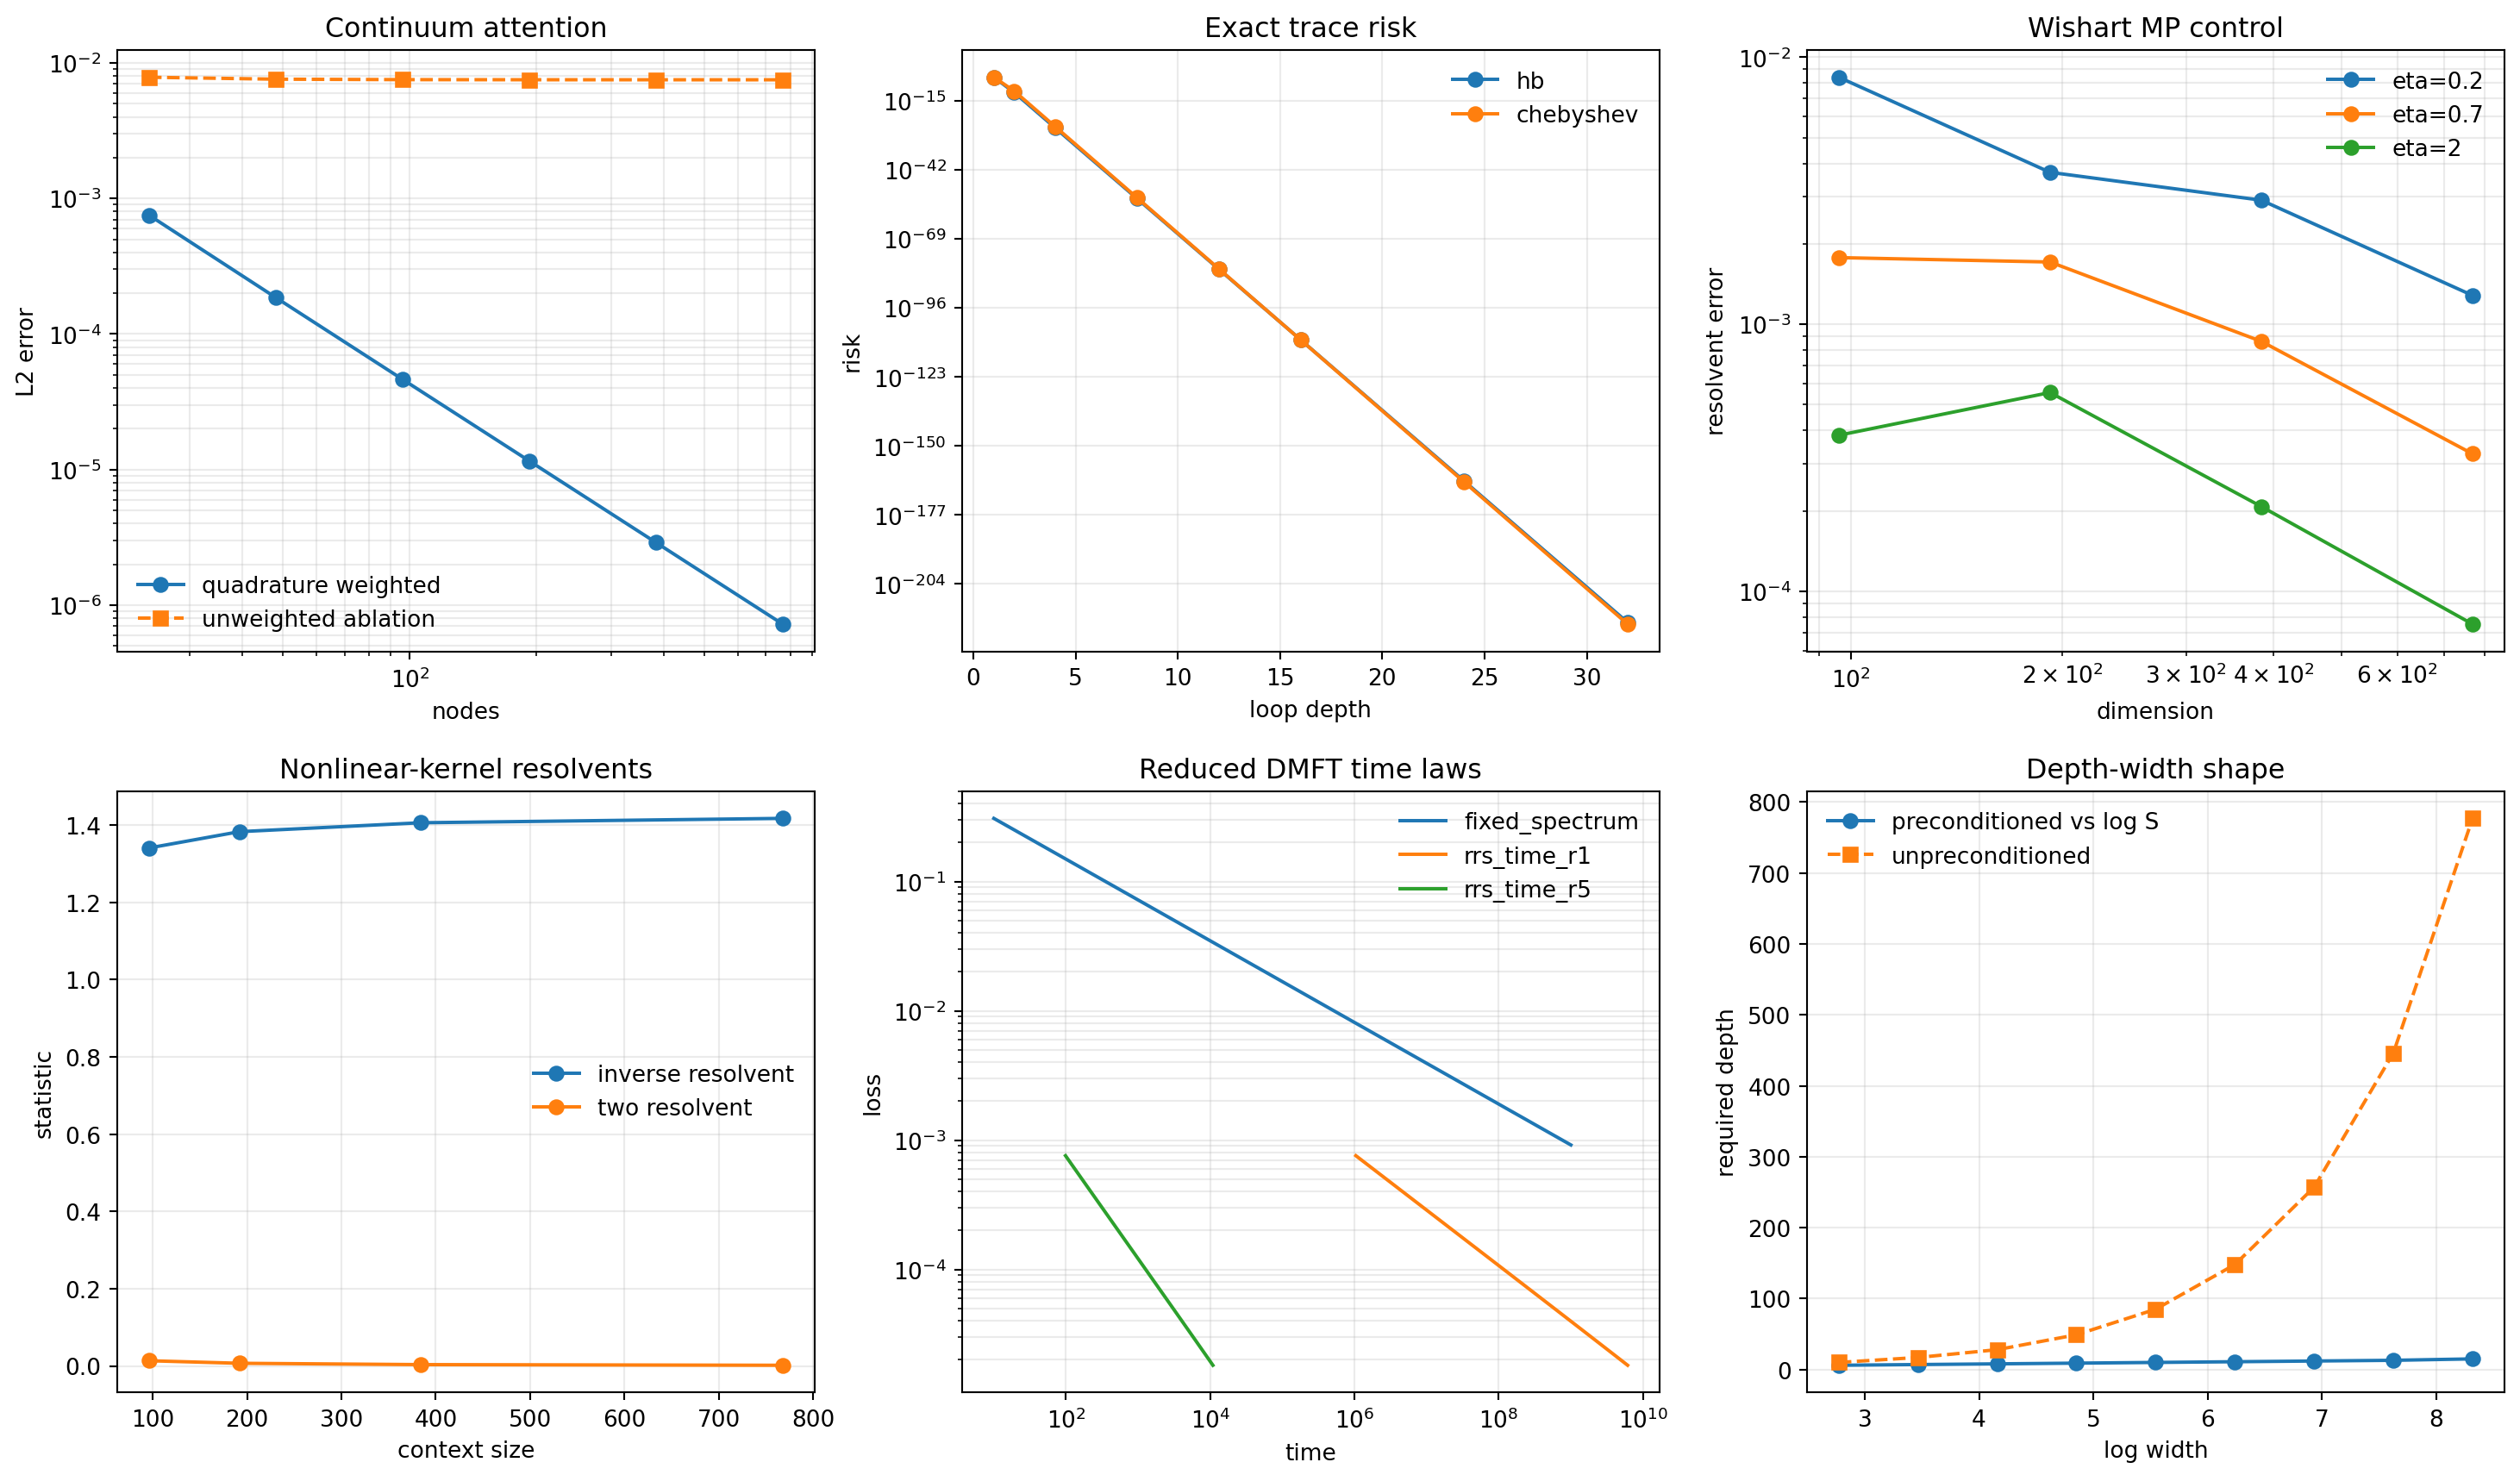
\includegraphics[width=0.98\linewidth]{experiments/transformers/kernel_matched_continuum_validation/results/theory/theory_validation_overview.png}
\caption{Algebraic, RMT, nonlinear-resolvent, reduced-DMFT, and
depth--width validations.  Marchenko--Pastur is shown only for the linear
control.}
\label{fig:theory-validation}
\end{figure}

\paragraph{Discretization covariance.}
On nonuniform meshes the lifted Ritz metric converges with fitted order
$2$ and
the transfer commutator with order
$2.437$.
Removing quadrature weights increases the finest-grid metric error by a factor
$4.037\times 10^{4}$.  This
directly separates continuum covariance from mere variable-length execution.

\begin{figure}[H]
\centering
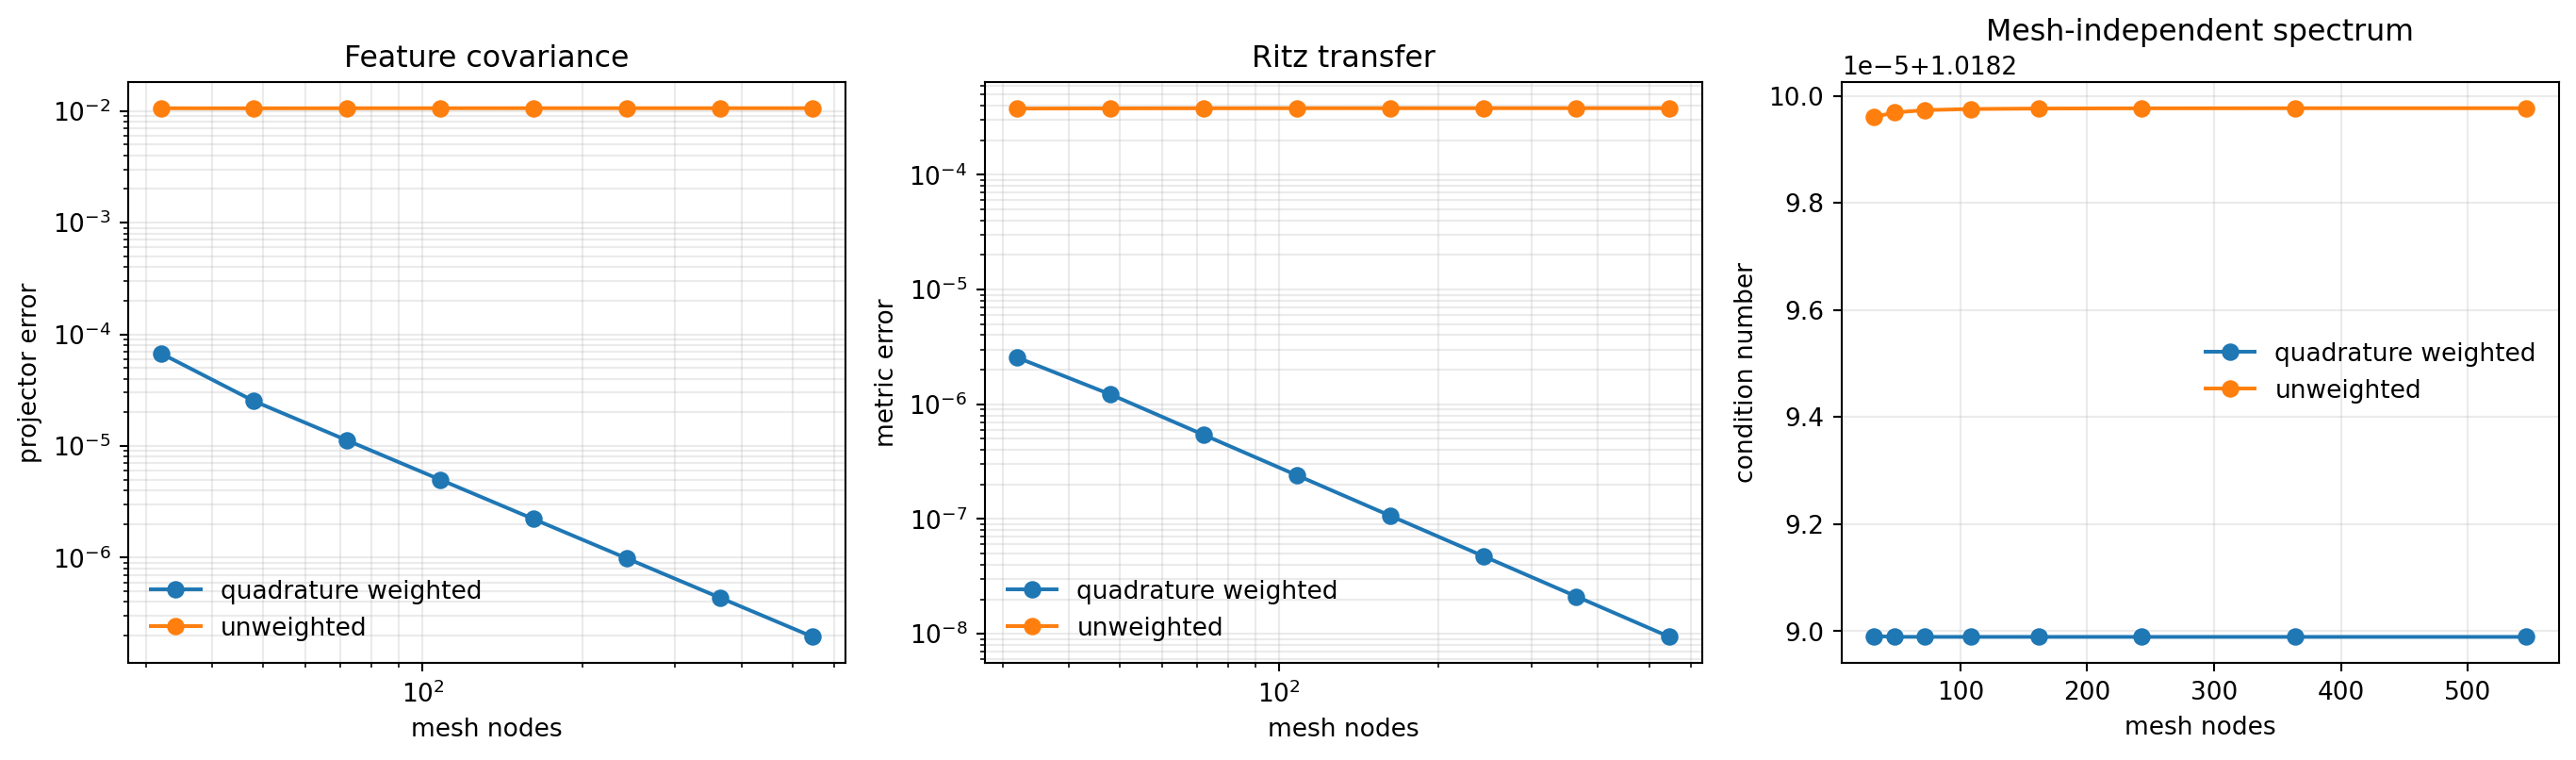
\includegraphics[width=0.82\linewidth]{experiments/transformers/kernel_matched_continuum_validation/results/discretization/discretization_validation.png}
\caption{Nonuniform-mesh transfer.  Quadrature weighting converges to one
lifted projector and Ritz metric, while the unweighted head retains a
sampling-measure bias.}
\label{fig:discretization-validation}
\end{figure}

\paragraph{Elliptic Bayesian inverse problem.}
We solve
$-\nabla\!\cdot(a_z\nabla u)+0.2u=m$ on the unit square with homogeneous
Dirichlet data.  The log-diffusion is a bounded random Fourier field and the
source covariance square root is
$W_z=\sigma_fI+\Phi_z\operatorname{diag}(d_z)\Phi_z^\top$, with a
task-dependent localized rank-24 component and a
nonzero floor.  Point observations and sparse elliptic solves produce the
prior-whitened posterior $H_z=I+U_zU_z^\top$.  The model-chosen RBF length
scale is compared with short- and long-scale ablations before one exact
block-power refinement and the Ritz construction.  The largest
standard sweep has $16384$ state unknowns and
$512$ observation tokens.  The contextual
kernel--Ritz metric reduces the effective condition number by a factor
$885.7$ and the
fixed four-HVP loops meet the common residual tolerance.  At this moderate
context, exact Woodbury is faster; its one-query total divided by kernel--HB is
$0.2137$.
Accordingly we make no universal speed claim against a structure-exploiting
Woodbury solve.

\begin{figure}[H]
\centering
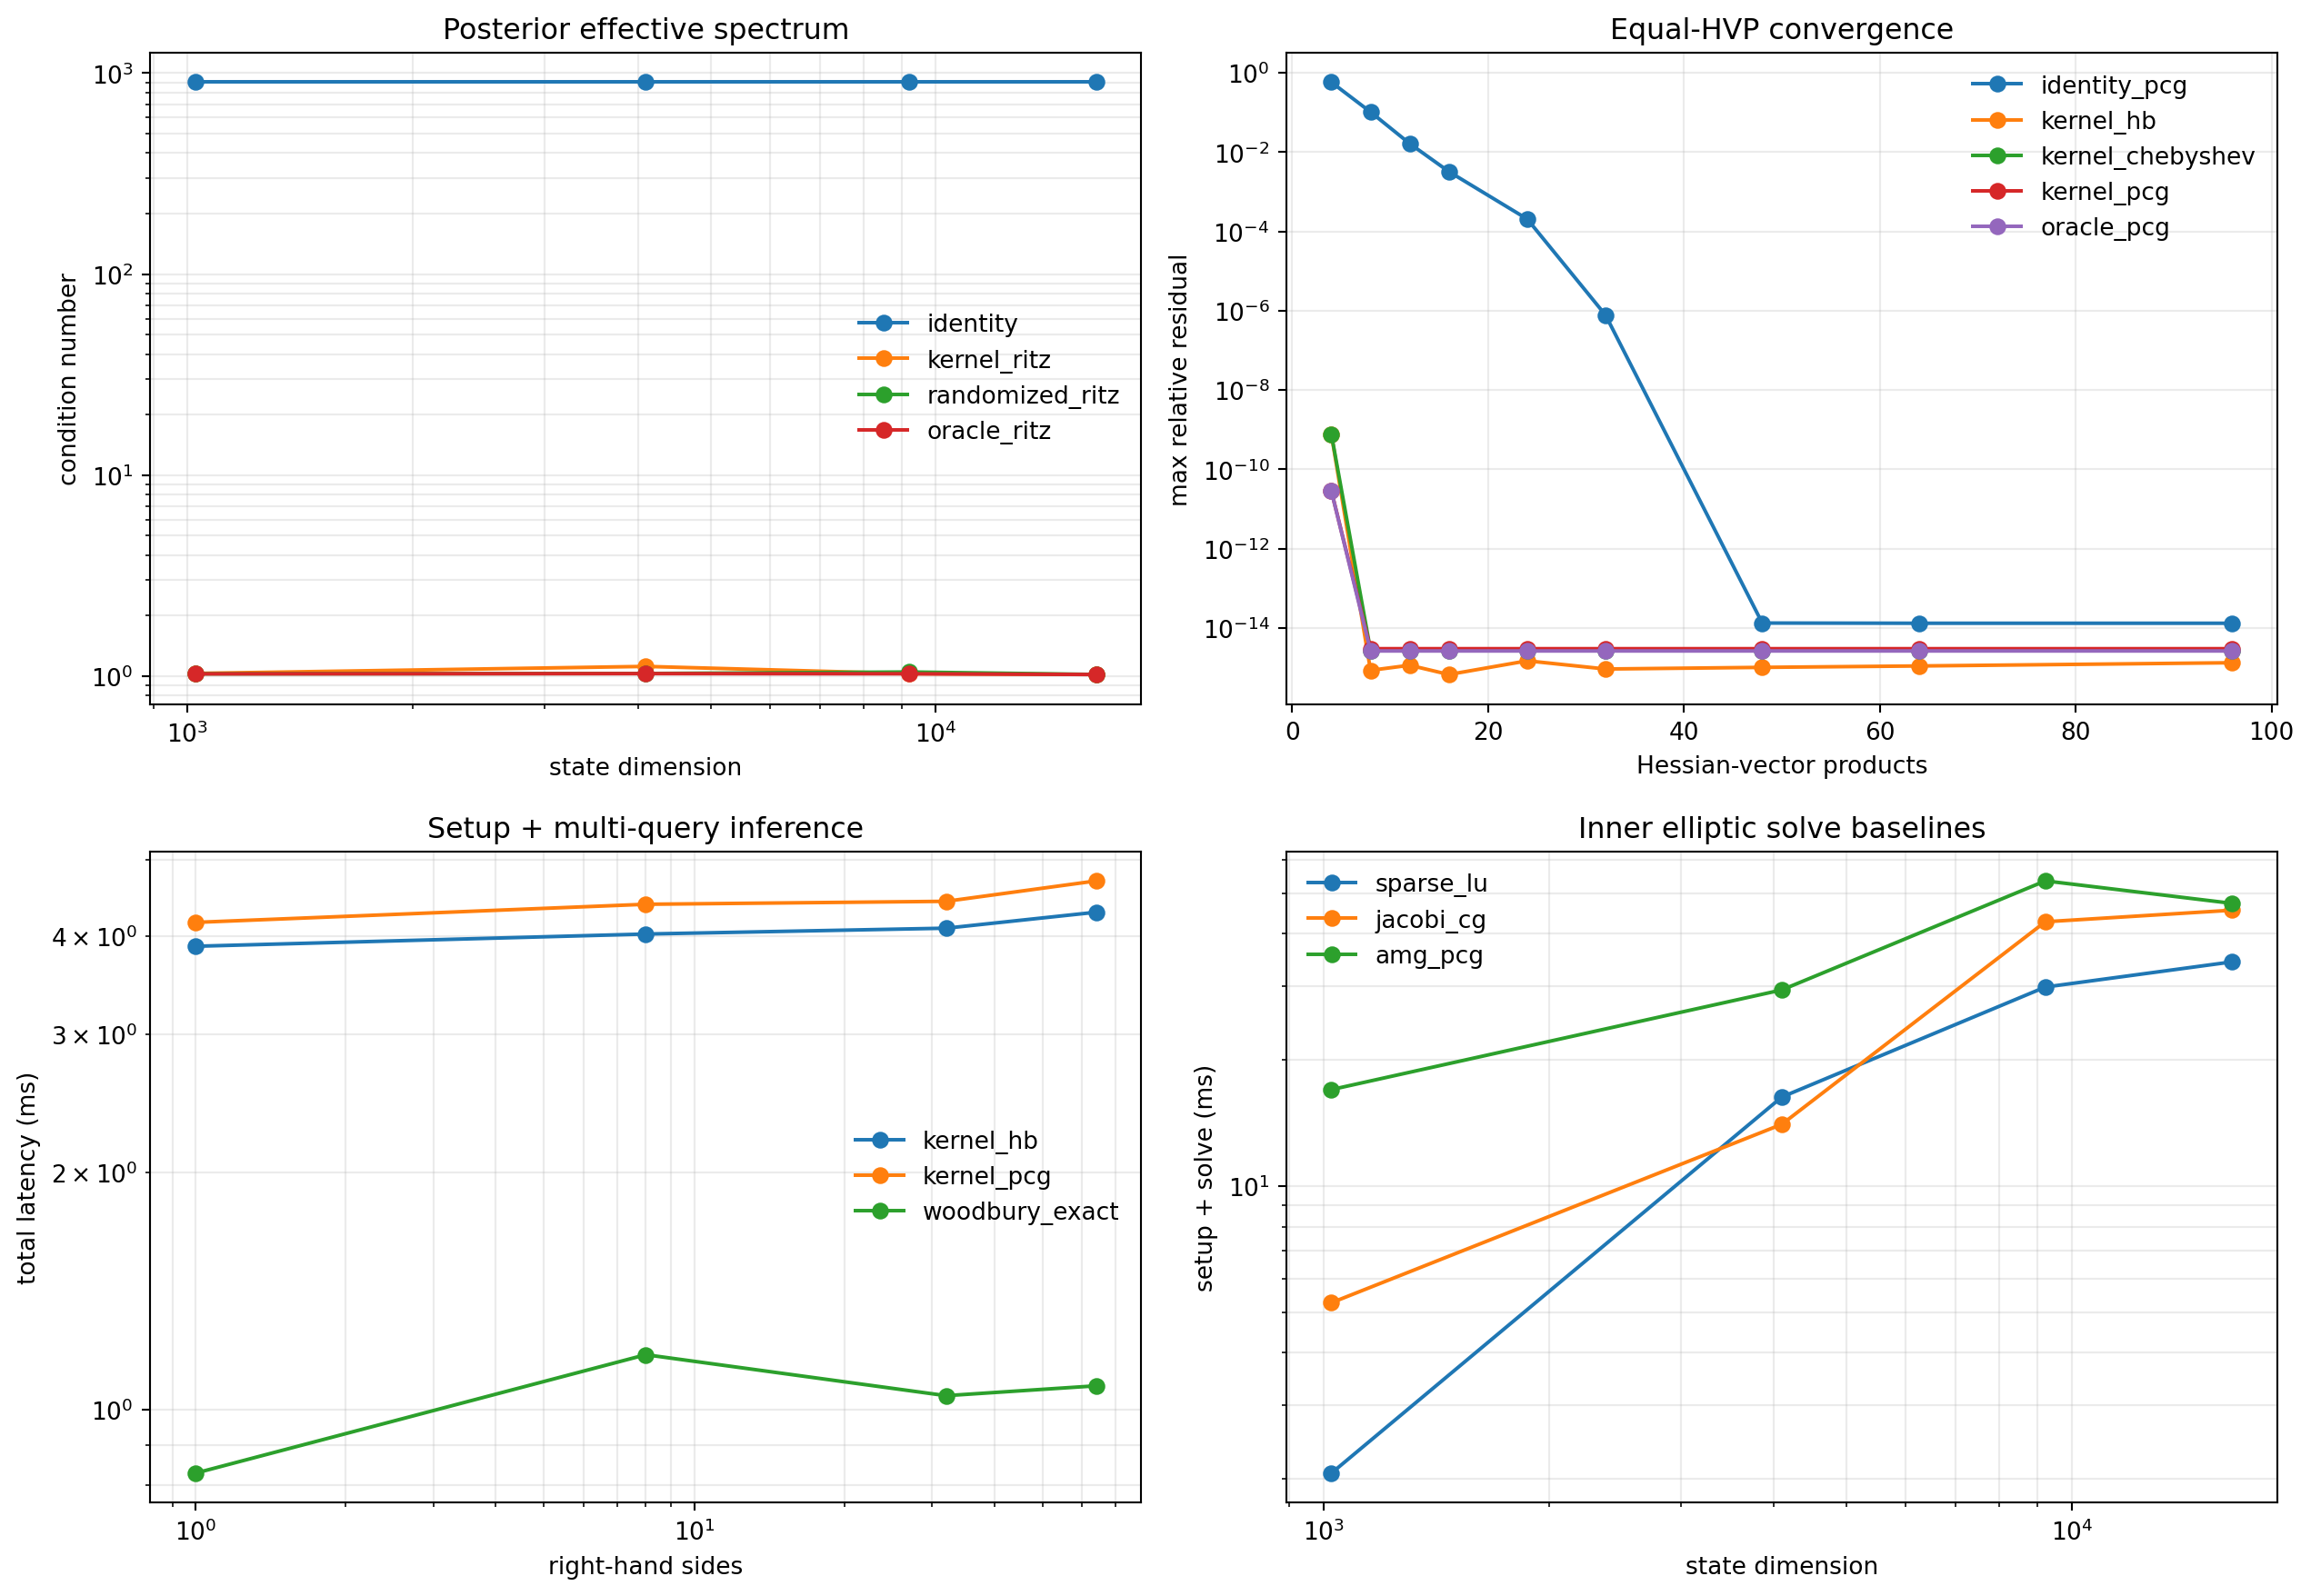
\includegraphics[width=0.90\linewidth]{experiments/transformers/kernel_matched_continuum_validation/results/pde/pde_validation_overview.png}
\caption{Variable-coefficient elliptic posterior validation: effective
spectra, equal-HVP convergence, multi-query timing, and sparse LU/Jacobi/AMG
inner PDE baselines.}
\label{fig:pde-validation}
\end{figure}

\begin{table}[H]
\centering
\caption{Long-context setup-plus-one-query latency on the same posterior
system on an NVIDIA H100 PCIe.  Parentheses give bootstrap 95\%
intervals from 11 repetitions.}
\label{tab:long-context-crossover}
\begin{tabular}{lrrr}
\toprule
Method & depth & latency (ms) & maximum relative residual\\
\midrule
Kernel--Ritz HB & 10 & 10.9
 [10.87,11.27]
 & $2.268\times 10^{-8}$\\
Exact Woodbury & --- & 24.03
 [23.38,24.26]
 & $1.541\times 10^{-15}$\\
Dense Cholesky & --- & 139.8
 [135.5,141.3]
 & $1.849\times 10^{-14}$\\
\bottomrule
\end{tabular}
\end{table}

At state dimension $N=16384$ and context length
$m=4096$, the measured dense/kernel median ratio is
$12.82$.
A nonoverlapping Woodbury crossover is also observed.
The admissible inference-speed statement is therefore restricted to the
measured context/query region and always includes feature construction.  PDE
assembly is a common context cost and is reported separately; AMG-PCG and
sparse LU are included as inner elliptic baselines.

\begin{figure}[H]
\centering
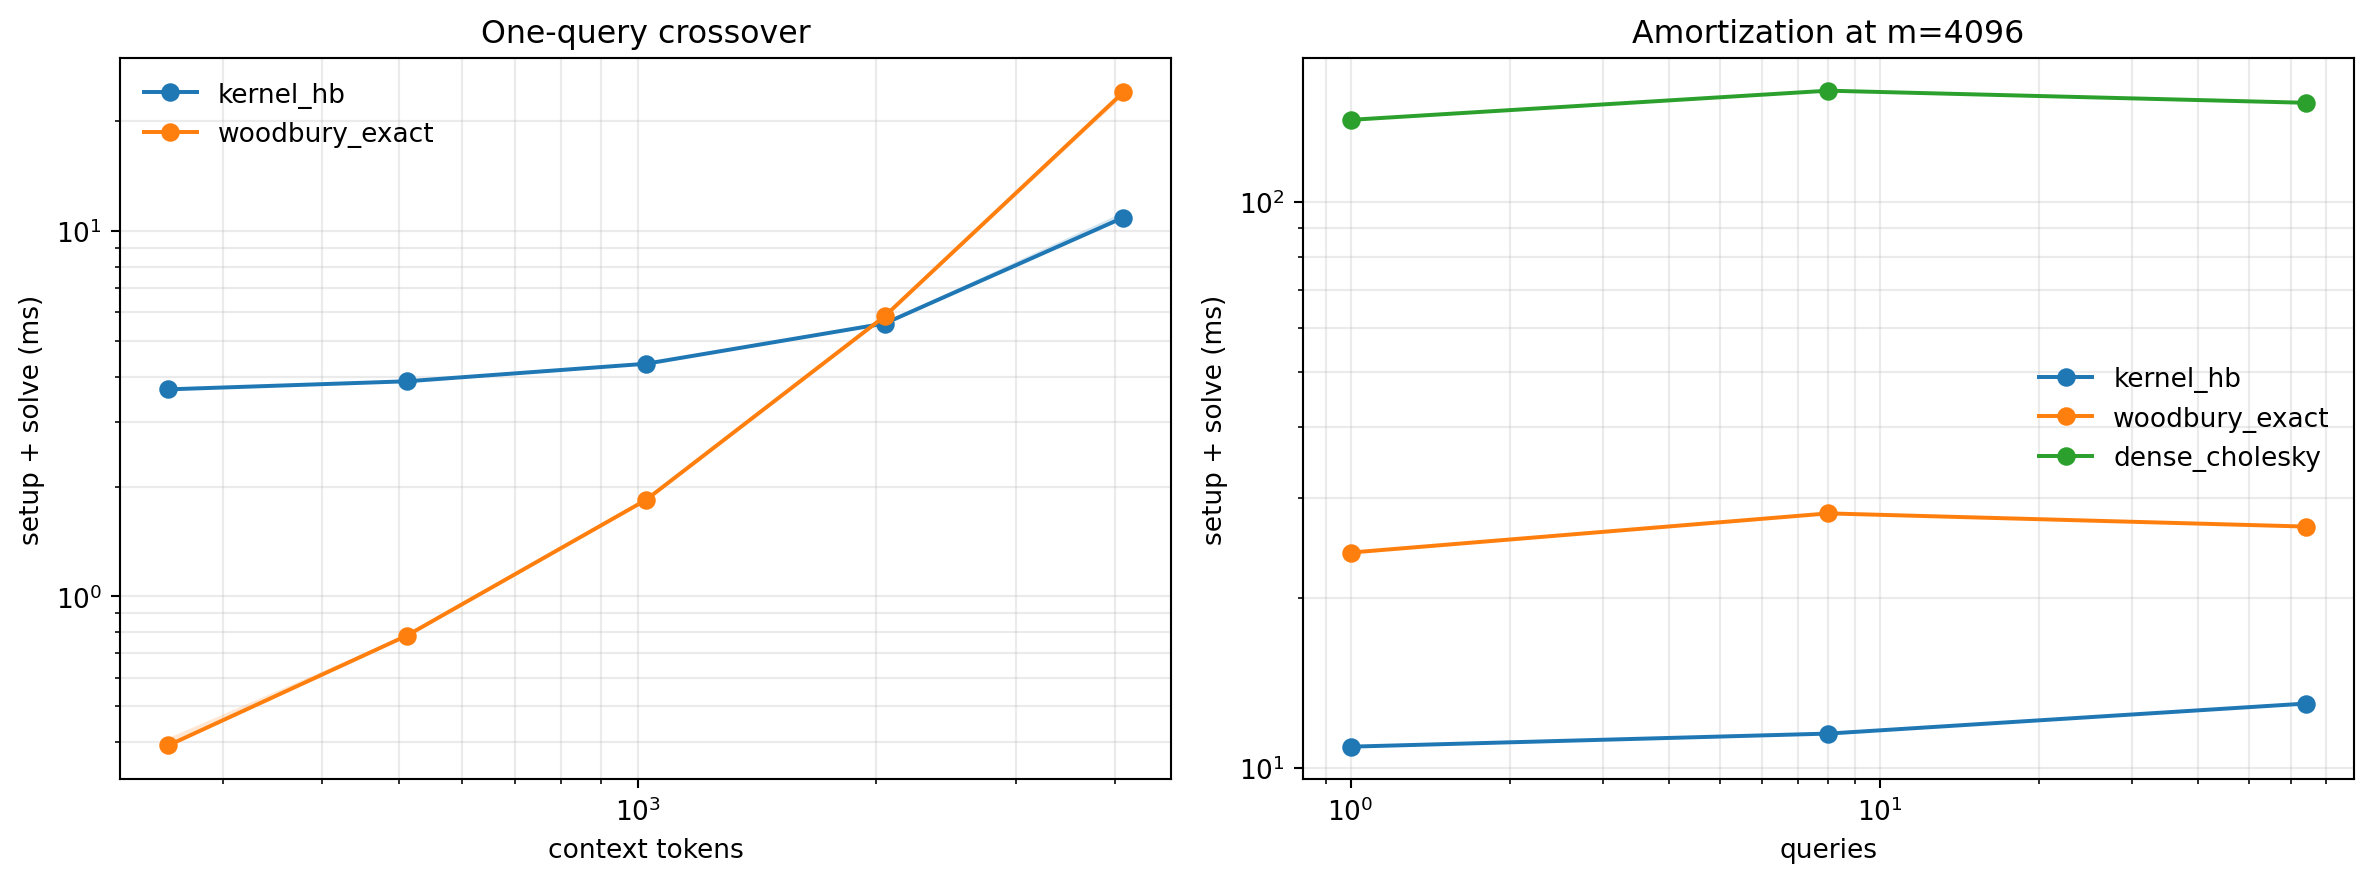
\includegraphics[width=0.82\linewidth]{experiments/transformers/kernel_matched_continuum_validation/results/crossover/long_context_crossover.png}
\caption{Setup-inclusive long-context crossover and multi-query
amortization.  Exact Woodbury is faster at short context; the compressed
kernel--Ritz loop crosses it only once the context is sufficiently long.}
\label{fig:long-context-crossover}
\end{figure}
\FloatBarrier


\section{Discussion and limitations}

\paragraph{The modelling choice.}
The kernel family and its geometry-defining hyperparameters are fixed.  This
matches a Bayesian analysis in which the prior has been specified before
inference.  Marginal-likelihood tuning, mixtures of kernels, or learned input
warps are valuable but distinct empirical-Bayes models; allowing them would
change the feature space during training and invalidate the clean resource
separation in Theorem~\ref{thm:master-risk}.

\paragraph{What is and is not learned.}
The encoder learns prompt-dependent coefficients and a finite subspace within
the prescribed feature geometry.  It does not learn the Hessian--vector
product, orthonormalization, projected inverse, Heavy--Ball arithmetic, or
Chebyshev recurrence.  This makes positivity and solver stability properties
of the architecture rather than regularization preferences.

\paragraph{Comparison to classical solvers.}
Finite elements, operator preconditioning, domain decomposition, and AMG can
already be mesh robust.  The proposed novelty is not irregular-mesh
competence.  It is amortized inference of a posterior metric from function
pairs rather than construction from a supplied system matrix, combined with
a discretization-covariance theorem and an exact loop.  Section
\ref{sec:numerical-validation} shows that runtime advantage only in a bounded
regime: for a long context and one or a few queries, the rank-$S$ contextual
metric avoids both an $N\times N$ Cholesky factorization and the
$m\times m$ Woodbury setup.  At moderate context exact Woodbury is faster, and
with enough repeated queries its setup can be amortized.  We therefore do not
claim universal domination of classical structure-exploiting solvers.

\paragraph{Limits of the scaling law.}
Equation \eqref{eq:master-risk} is exact in the commuting Gaussian sequence
model.  Applying the same exponents to random-design, noncommuting, or fully
feature-learning Transformers needs additional concentration, random-matrix,
or DMFT analysis.  The deterministic trace formula
\eqref{eq:trace-risk} states precisely what such an analysis must supply: the
weighted spectral law of the prompt-conditioned preconditioned Hessian.

\clearpage
\section{Conclusion}

The nonlinearity of attention should reflect the covariance geometry assumed
by the modeller.  Exponential softmax is the correct normalized interaction
for an RBF-type kernel with fixed scale; it is not a universal representation
of Gaussian-process covariance.  Once quadrature and normalization are made
explicit, kernel attention becomes a consistent continuum operation.  Its
contextual outputs can be converted by exact Ritz algebra into an SPD
approximation of posterior covariance, after which tied Heavy--Ball or
Chebyshev layers perform auditable inference.  The resulting theory separates
five resources---context, width, training time, depth, and discretization---and
shows how mesh-independent posterior geometry yields mesh-independent looped
inference.  The numerical audit supports the exact spectral and reduced-model
predictions, rejects importing the linear Marchenko--Pastur law into nonlinear
softmax, and locates a setup-inclusive long-context crossover against both
dense Cholesky and exact Woodbury.  This measured boundary is part of the
claim: outside it, the appropriate classical solver should be used.

\clearpage
\appendix

\section{Proofs for continuum kernel attention}

\begin{proof}[Proof of Proposition~\ref{prop:reversibility}]
For $f,g\in L^2(\pi_\kappa)$, Fubini's theorem and symmetry give
\begin{align*}
 \langle f,\calA_\kappa g\rangle_{L^2(\pi_\kappa)}
 &=\frac1{Z_\kappa}\int_X\int_X
 f(x)\kappa(x,y)g(y)\rho(\dd y)\rho(\dd x)\\
 &=\langle\calA_\kappa f,g\rangle_{L^2(\pi_\kappa)}.
\end{align*}
Taking $f=g$ shows nonnegativity whenever $\kappa$ is a positive-semidefinite
integral kernel.  Discretely,
\[
 \pi_{h,i}a_{ij}^{\kappa,h}
 \propto\omega_i\omega_j\kappa(x_i,x_j)
 =\pi_{h,j}a_{ji}^{\kappa,h},
\]
which is detailed balance.  The same quadratic-form calculation proves
positivity.
\end{proof}

\begin{proof}[Proof of Theorem~\ref{thm:continuum-consistency}]
Write $N(x)=\int\kappa(x,y)v(y)\rho(\dd y)$ and
$D(x)=d_\kappa(x)$, with quadrature approximations $N_h,D_h$.  Assumption
\ref{ass:quadrature} gives $|N_h-N|\le C_vh^p$ and
$|D_h-D|\le C_0h^p$.  For sufficiently small $h$, $D_h\ge d_0/2$.  Hence
\[
 \left|\frac{N_h}{D_h}-\frac ND\right|
 \le\frac{|N_h-N|}{|D_h|}
 +\frac{|N|\,|D_h-D|}{|D_h|D}
 \le C(1+\|v\|_\infty)h^p.
\]
The finitely many coarser admissible discretizations are absorbed by enlarging
$C$.
\end{proof}

\section{Proofs for the posterior metric}

\begin{proof}[Proof of Proposition~\ref{prop:spd}]
Every $x\in\calU$ decomposes as $x=Qa+x_\perp$ with $Q^*x_\perp=0$.  Since
$H\succeq I$,
\[
 \langle x,B_Qx\rangle
 =\|x_\perp\|^2+
 \langle a,(Q^*HQ)^{-1}a\rangle>0
\]
for $x\ne0$, and $(Q^*HQ)^{-1}\preceq I$ proves $B_Q\preceq I$.
If $\range(A)\subseteq\range(Q)$, both $\range(Q)$ and its orthogonal
complement are invariant under $H$.  On the complement $H=I$, while on
$\range(Q)$ the second term in \eqref{eq:ritz-metric} is the exact inverse of
the restriction.  Thus $B_Q=H^{-1}$.  Rearranging
\eqref{eq:ritz-metric} gives \eqref{eq:negative-correction}; the bracket is
positive semidefinite because $Q^*HQ\succeq I$.
\end{proof}

\begin{lemma}[Ritz map perturbation]
\label{lem:ritz-perturbation}
Let $I\preceq H_1,H_2\preceq MI$ and let $P_i=Q_iQ_i^*$ be rank-$S$
orthogonal projectors.  After optimal right-orthogonal alignment of $Q_1,Q_2$,
\begin{equation}
 \|B(H_1,Q_1)-B(H_2,Q_2)\|_\op
 \le \|H_1-H_2\|_\op+C_M\|P_1-P_2\|_\op,
 \label{eq:ritz-lipschitz}
\end{equation}
where $B(H,Q)$ denotes \eqref{eq:ritz-metric} and $C_M$ may be chosen as in
\eqref{eq:tail-constants} after increasing it by an absolute constant.
\end{lemma}

\begin{proof}
The principal-angle relation gives an alignment with
$\|Q_1-Q_2\|_\op\le\sqrt2\|P_1-P_2\|_\op$.  Add and subtract the two
complementary projectors and the two Ritz terms.  The resolvent identity
\[
 R_1^{-1}-R_2^{-1}=R_1^{-1}(R_2-R_1)R_2^{-1},
 \qquad R_i=Q_i^*H_iQ_i,
\]
has $\|R_i^{-1}\|\le1$.  Moreover
\[
 \|R_1-R_2\|
 \le\|H_1-H_2\|+2M\|Q_1-Q_2\|.
\]
The outer factors contribute another $2\|Q_1-Q_2\|$, and the complementary
projectors contribute $\|P_1-P_2\|$.  Combining the bounds proves
\eqref{eq:ritz-lipschitz} with the advertised nonoptimal constant.
\end{proof}

\begin{proof}[Proof of Theorem~\ref{thm:subspace-spectrum}]
Let $Q_\star$ span the first $S$ eigenvectors.  The spectral theorem gives
\[
 \|B_{Q_\star}-H^{-1}\|_\op
 =\sup_{j>S}\left|1-\frac1{1+\nu_j}\right|=r_S.
\]
Lemma~\ref{lem:ritz-perturbation} with $H_1=H_2=H$ gives
$\|B_Q-B_{Q_\star}\|\le C_M\delta_S$.  This proves
\eqref{eq:inverse-approximation}.  Consequently
\[
 \|H^{1/2}B_QH^{1/2}-I\|_\op
 \le M(r_S+C_M\delta_S)=\epsilon_S.
\]
Weyl's inequality places the spectrum of $H^{1/2}B_QH^{1/2}$ in the stated
interval.  It has the same spectrum as $B_Q^{1/2}HB_Q^{1/2}$, which proves
\eqref{eq:spectral-equivalence}.
\end{proof}

\begin{proof}[Proof of Theorem~\ref{thm:discretization-covariance}]
Apply Lemma~\ref{lem:ritz-perturbation} to $(\bar H_h,\bar P_h)$ and $(H,P)$,
then use \eqref{eq:operator-consistency}; this gives
\eqref{eq:lift-convergence}.  Insert and subtract the continuum $B$ between
the two lifted discrete metrics.  The triangle inequality gives the sum of
the two one-level errors.  Compressing back to the two discrete spaces yields
\eqref{eq:commutator-bound}; any failure of the transfer to equal exact lifted
compression is, by definition, $\eps_{\rm tr}$.
\end{proof}

\begin{proof}[Proof of Corollary~\ref{cor:mesh-independent}]
Theorem~\ref{thm:discretization-covariance} and
\eqref{eq:operator-consistency} bound the lifted symmetrically preconditioned
perturbation by a term tending to an encoder-dependent floor.  By hypothesis
that floor is below $\mu_0/2$, and $h$ can be chosen so that the full
perturbation remains below $\mu_0/2$.  Spectra of bounded self-adjoint
operators are stable under operator-norm perturbations; one may then take
$\mu=\mu_0/2$ and enlarge $L_0$ by the same uniform perturbation bound.
\end{proof}

\section{Proofs for looped inference}

\begin{proof}[Proof of Theorem~\ref{thm:hb}]
Let $e_\ell=x_\ell-x_\star$ and
$\wt e_\ell=B^{-1/2}e_\ell$.  Then
\[
 \wt e_{\ell+1}=\bigl[(1+\beta)I-\alpha K\bigr]\wt e_\ell
 -\beta\wt e_{\ell-1},
\]
so $\wt e_\ell=p_\ell(K)\wt e_0$.  For the coefficients
\eqref{eq:hb-coefficients}, write
$1+\beta_\star-\alpha_\star z=2q\tau$, where $\tau\in[-1,1]$ as
$z$ ranges over $[\mu,L]$.  Setting $s_\ell=p_\ell/q^\ell$ gives
$s_{\ell+1}=2\tau s_\ell-s_{\ell-1}$ and hence
\[
 p_\ell(z)=q^\ell\bigl[U_\ell(\tau)-qU_{\ell-1}(\tau)\bigr].
\]
Since $|U_\ell(\tau)|\le\ell+1$ on $[-1,1]$,
\[
 \max_{z\in[\mu,L]}|p_\ell(z)|
 \le[1+\ell(1+q)]q^\ell.
\]
Functional calculus proves \eqref{eq:hb-bound}.  The strict stability region
\eqref{eq:jury} follows from the Jury conditions for
$r^2-(1+\beta-\alpha z)r+\beta$, uniformly over $z\in[\mu,L]$.
\end{proof}

\begin{proof}[Proof of Proposition~\ref{prop:trace-risk}]
In the variable $u=B^{-1/2}x$, the exact solution is $u_\star=K^{-1}c$ and a
fixed polynomial method has error $p_\ell(K)u_\star$.  Therefore
\[
 \|x_\ell-x_\star\|_H^2
 =\langle p_\ell(K)K^{-1}c,
 Kp_\ell(K)K^{-1}c\rangle
 =\langle c,K^{-1}p_\ell(K)^2c\rangle.
\]
Taking the conditional expectation gives the trace.  The final expression is
the spectral theorem applied to the positive weighted measure
$\nu_c(E)=\tr(\Sigma_c\mathbf 1_E(K))$.
\end{proof}

\section{Proofs for the reduced preconditioner operator calculus}

\begin{proof}[Proof of Proposition~\ref{prop:kernel-iso}]
Conjugation invariance of the population loss implies that its gradient at a
scalar operator is scalar.  Zero initialization therefore leaves the scalar
manifold invariant.  Conditional on $\widehat T_{\kappa,n}$, spectral calculus
turns the normalized trace loss into the empirical average of
$(1-L_d^{-1}\gamma\lambda)^{2L_d}$.  Differentiating gives the empirical
version of \eqref{eq:kernel-iso-flow}.  Convergence of the empirical spectral
measure, together with uniform integrability on the stable parameter range,
gives \eqref{eq:kernel-iso-flow}--\eqref{eq:kernel-iso-loss}.
\end{proof}

\begin{proof}[Proof of Proposition~\ref{prop:fs-flow}]
Simultaneous diagonalization turns \eqref{eq:reduced-gamma-loss} into
\[
 \loss_{L_d}=\sum_j\omega_j\lambda_j
 \left(1-L_d^{-1}\lambda_j\gamma_j\right)^{2L_d}.
\]
Differentiation gives \eqref{eq:fs-modal-flow}, up to the stated constant
rescaling of time.  The zero of each represented residual is
$\gamma_j=L_d/\lambda_j$.  As $L_d\to\infty$,
$(1-L_d^{-1}\lambda_j\gamma_j)^{2L_d-1}\to
e^{-2\lambda_j\gamma_j}$.  With the factor-two convention,
\[
 \dot\gamma_j=2\omega_j\lambda_j^2e^{-2\lambda_j\gamma_j}.
\]
Multiplying by $e^{2\lambda_j\gamma_j}$ and integrating from zero gives
$e^{2\lambda_j\gamma_j(t)}=1+4\omega_j\lambda_j^3t$.  Substitution in the
modal loss proves \eqref{eq:fs-exact-flow}.
\end{proof}

\begin{proof}[Proof of Corollary~\ref{cor:fs-regular-variation}]
Integral comparison for regularly varying sequences reduces the asymptotic,
up to positive constants, to
\[
 \int_1^\infty\frac{x^{-s}}{1+t x^{-r}}\,\dd x.
\]
The substitution $x=t^{1/r}u$ gives
$t^{-(s-1)/r}$ times an integral converging at both zero and infinity exactly
when $r>s-1>0$.  This proves \eqref{eq:fs-time-power}.  Under the displayed
source condition, Karamata's theorem gives
$a_j\asymp j^{-\nu\beta-1}$; multiplying by $\lambda_j^2$ gives
$b_j\asymp j^{-(\nu\beta+1+2\nu)}$.
\end{proof}

\begin{proof}[Proof of Proposition~\ref{prop:rrs-laws}]
At infinite depth,
\[
 \loss_\infty(\gamma)=
 \sum_j a_je^{-2\gamma\lambda_j},
 \qquad a_j=\omega_j\lambda_j.
\]
Let $J_\gamma=\lfloor\gamma^{1/\nu}\rfloor$.  Modes
$j\gg J_\gamma$ have $\gamma\lambda_j=O(1)$ and contribute a constant
fraction of their tail energy, which is $\Theta(J_\gamma^{-\nu\beta})$.
Modes $j\ll J_\gamma$ are exponentially suppressed; a dyadic decomposition
around $J_\gamma$ bounds their total by the same order.  Hence
$\loss_\infty(\gamma)=\Theta(\gamma^{-\beta})$.  Differentiating the
modal sum, or repeating the cutoff argument for the derivative, gives
$\dot\gamma=\Theta(\gamma^{-\beta-1})$ under gradient flow.  Integration
yields \eqref{eq:rrs-time-law}.

For finite depth, stability along the top eigendirection restricts
$\gamma<2L_d/\lambda_1$.  Choosing $\gamma=cL_d$ with fixed admissible $c>0$
gives the upper bound $O(L_d^{-\beta})$ by the same cutoff argument.  Conversely,
every stable choice has $\gamma=O(L_d)$, so modes
$j\gtrsim L_d^{1/\nu}$ retain a constant fraction of their energy and give the
matching lower bound.  A spectral rank-$S$ projection and an idealized
context revealing the first $n$ modes leave the tails beyond $S$ and $n$,
respectively;
\eqref{eq:rrs-source-capacity} gives their stated orders.
\end{proof}

\begin{proof}[Proof of Proposition~\ref{prop:amplitude-parameterization}]
Since $\gamma=w^r$, gradient flow in $w$ gives
\[
 \dot\gamma
 =r w^{r-1}\dot w
 =-r^2w^{2r-2}\loss'(\gamma)
 =-r^2\gamma^{2-2/r}\loss'(\gamma).
\]
When $\loss(\gamma)\asymp\gamma^{-\beta}$, this is
$\dot\gamma\asymp\gamma^{1-2/r-\beta}$.  Integration gives
$\gamma^{\beta+2/r}\asymp t$, and substitution into the loss proves
\eqref{eq:parameterized-time-law}.
\end{proof}

\paragraph{Derivation of the two-point formula.}
Cauchy's functional calculus gives
\[
 p(M)=\frac{1}{2\pi i}\oint_{\mathcal C}
 p(z)(zI-M)^{-1}\,\dd z.
\]
Insert this representation for both polynomial factors in the quadratic risk,
use Fubini's theorem, and take the trace cyclically.  This gives
\eqref{eq:two-point-kernel-resolvent}.  Balancing
$S^{-\nu\beta}$ with $L_d^{-\beta}$ gives
\eqref{eq:original-shape}; balancing it with $q^{2L_d}$ gives
\eqref{eq:preconditioned-shape}.  The Heavy--Ball prefactor changes only the
lower-order $\log\log S$ term.

\section{Proofs for the scaling laws}

\begin{proof}[Proof of Theorem~\ref{thm:master-risk}]
Conditioning on $Y_j$, decompose
\[
 f_j-\wh f_{L,j}
 =f_j-\E[f_j\mid Y_j]
 +\E[f_j\mid Y_j]-\wh f_{L,j}.
\]
The two terms are orthogonal in $L^2$ by the defining property of conditional
expectation.  Their variances are $r_{n,j}$ and
\[
 \left[1-(1-p_L(\zeta_{h,j}))\chi_j(t)\right]^2v_{n,j}
\]
for $j\le M_h$.  For $j>M_h$ the estimator is zero and the risk is
$\lambda_j$.  Summing independent modes proves \eqref{eq:master-risk}.  The
$h^{2p}$ perturbation follows from the assumed squared-risk stability of the
represented modes.
\end{proof}

\begin{proof}[Proof of Theorem~\ref{thm:marginal-scaling}]
For the context term, regular variation and an integral comparison give
\begin{align*}
 \sum_j\frac{\sigma^2\lambda_j}{\sigma^2+n\lambda_j}
 &\sim\int_0^\infty
 \frac{c_\lambda}{x^a+nc_\lambda/\sigma^2}\,\dd x\\
 &=c_\lambda^{1/a}
 \left(\frac{\sigma^2}{n}\right)^{1-1/a}
 \int_0^\infty\frac{\dd u}{1+u^a}.
\end{align*}
The last integral is $\pi/[a\sin(\pi/a)]$.  The width law is the standard
tail asymptotic for a regularly varying sequence.  Similarly,
\begin{align*}
 \sum_jw_je^{-2\gamma_jt}
 &\sim c_w\int_0^\infty x^{-c}
 e^{-2c_\gamma t x^{-b}}\,\dd x\\
 &=\frac{c_w}{b}(2c_\gamma t)^{-(c-1)/b}
 \Gamma\!\left(\frac{c-1}{b}\right).
\end{align*}
Finally apply Theorem~\ref{thm:hb} and
\eqref{eq:chebyshev-bound} modewise in
\eqref{eq:master-risk}; the represented posterior-mean variance has finite
trace, which is absorbed into $C$.
\end{proof}

\begin{proof}[Proof of Proposition~\ref{prop:random-rotations}]
The objective \eqref{eq:global-inverse-risk} is a strictly convex quadratic in
$B$, hence its unique minimizer is $\E_UH_U^{-1}$.  Haar invariance implies
$V(\E_UH_U^{-1})V^\top=\E_UH_U^{-1}$ for every orthogonal $V$, so the
expectation is a scalar multiple of the identity.  Its trace determines the
scalar and gives \eqref{eq:isotropic-global-head}.
\end{proof}

\section{Comment on the nonlinear outer iteration}

\begin{proof}[Justification of Proposition~\ref{prop:gauss-newton}]
Uniform spectral equivalence puts every symmetrically preconditioned $H_k$ in
one interval $[\mu,L]$.  Theorem~\ref{thm:hb} or
\eqref{eq:chebyshev-bound} therefore yields a depth depending only on the
desired forcing tolerance and on $L/\mu$, not on the mesh.  Once
\eqref{eq:forcing-condition} holds, the update is an ordinary inexact
Gauss--Newton step.  The asserted local conclusions are the standard
contraction estimates obtained by combining Jacobian Lipschitz continuity,
uniform coercivity, and the forcing sequence; the learned metric affects only
the cost of reaching the prescribed inner residual.
\end{proof}

\bibliographystyle{plainnat}
\begingroup
\small
\bibliography{kernel_matched_continuum_looped_gp}
\endgroup

\end{document}
